\documentclass{report}

\usepackage[utf8]{inputenc}
\usepackage[T1]{fontenc}
\usepackage[francais]{babel}
\usepackage[Lenny]{fncychap} %Sonny, Lenny, Glenn, Conny, Rejne, Bjarne, Bjornstrup
\usepackage{mathpazo}
\usepackage{wrapfig}
\usepackage{graphicx}
\usepackage{soul}
\usepackage[colorlinks=true, linkcolor=blue]{hyperref}
\usepackage[a4paper, width=180mm, top=25mm, bottom=25mm]{geometry}
\usepackage{parskip}
\usepackage{enumitem}
\usepackage{titlesec}
\usepackage[final]{pdfpages}
\setlist[itemize]{label=\textbullet}
\usepackage{fancyhdr}
\usepackage{amssymb}
\pagestyle{fancy}
\fancyhead{}
\fancyhead[C]{\leftmark}
\renewcommand{\headrulewidth}{0.4pt}
\renewcommand{\footrulewidth}{0.4pt}
\usepackage{multirow} % Assurez-vous que cette ligne est présente
\usepackage{csquotes}

\begin{document}

\includepdf[pages=1]{Page_garde.pdf} 

\pagenumbering{gobble}

%Sommaire
\renewcommand{\contentsname}{Sommaire}
\tableofcontents
%\includepdf[pages=7-8]{tables/withFigure.pdf}


%les remerciements
\chapter*{Remerciements}
\Large
%\setlength{\parindent}{0.5cm} 
Avant tout, Il semble approprié d'entamer ce mémoire par des remerciements, d’abord au bon dieu de nous avoir accordé la force et le courage de mener à terme ce modeste travail.\\

Toute notre reconnaissance et toute notre gratitude vont vers Mr Kacem CHERFA, notre promoteur, qui nous a aidé et accompagné tout au long de cette expérience professionnelle avec beaucoup de patience et d'enthousiasme.\\

Nos profondes remerciements s’adressent à Mme Lamia BERKANI, notre enseignante à l'USTHB, de nous avoir guidé et orienté durant les différentes étapes de ce projet avec ça pédagogie et ça ferveur.\\

Nous remercions également les membres du jury d’avoir accepté d’examiner et de juger notre travail.\\

Que tous ceux qui, de près ou de loin ont contribué, par leurs conseils, leurs
encouragements ou leur amitié à l’aboutissement de ce travail, trouvent ici
l’expression de notre profonde reconnaissance.\\

Pour leur encouragement, leur soutien moral et la patience qu’ils nous ont
manifestée durant toute l’année, nous remercions fortement tous les membres de
nos familles.\\

Enfin remercier nos parents serait se répéter, parfois pour exprimer plus que ce qu’on a envie de dire on a recours au silence.

\normalsize
%\noindent
%les résumé
\chapter*{Résumé}
Le présent mémoire rend compte de notre projet de fin d’études au sein de COSIDER CANALISATIONS et au département Informatique de l’Université des Sciences et de la Technologie Houari Boumediene.\\ Il
s’agit de concevoir et de développer un système de gestion pour la direction des approvisionnements et de la sous-traitance DAST, qui se trouve face à plusieurs problèmes de gestion.\\
Notre solution informatique est une application web riche en fonctionnalités, accessible et parfaitement adaptée aux besoins des employés.\\
Certaines technologies et librairies sont employées et plusieurs langages de programmations tels que le \emph{php}, le \emph{XML} ou le \emph{JavaScript} ont été utilisées. Une base de données relationnelles pour modéliser les informations est également mise en place.\\
Le déroulement du projet s‘est effectué suivant trois étapes :
\begin{itemize}
    \item Étude approfondie de l'existant dans l'entreprise,
    \item Conception et modélisation du système,
    \item Réalisation de l'application tout en respectant les objectifs prédéfinis.
\end{itemize}
\vspace*{1cm}
Mots clés : S.I , UML , Application Web , Apache , MySql , 
%le résumé en langue Anglaise
\chapter*{Abstract}
The present dissertation of our graduation project within COSIDAR CANALISATIONS and the departement
of computer science of the univeristy of science and technology houari boumadien.\\
It’s about conceiving and developping a managemenent system for the direction of supplies and subcontacting DAST which is facing several management problems.\\
Our IT solution is a rich web app , accessible and perfectly adapted to the needs of the employees.
Some technologies and libraries are employed and differents programming languages such
the \emph{PHP}, \emph{XML} and \emph{JavaScript} were used. A relational database is also introduced.\\
The project progress went through three major steps :
\begin{itemize} 
       \item A depth study of the existing within the enterprise,
       \item Design and system modeling,
       \item Realisation of the app while respecting the defined objectives.
\end{itemize}
\vspace*{1cm}
key words : S.I , UML , Web Application , Apache , MySql


%liste des figures\listoffigures
%liste des tableaux\listoftables
%introduction generale
\chapter*{Introduction générale}
\pagenumbering{arabic}
L’informatique est un domaine d'activité scientifique, technique et industriel dont les champs d'application ne cessent de se développer.
Elle a progressé plus que toutes autres disciplines, d’ailleurs, elle est au cœur des plus grandes innovations des 50 dernières années.

Dans les entreprises, l’informatique et ses différentes activités sont devenues un outil clé de la performance des processus, de la qualité des produits et de la sécurité du parc informationnel.

Pour la plus part des entreprises du 21 éme siècle, l'information est considérée comme la principale ressource de créativité, cela est possible grâce à l'outil informatique utilisé de plus en plus pour le stockage, l'analyse et la transmission de cette ressource incontournable.

Les entreprises algériennes ont déjà pris conscience de ces avancés technologiques et de l'importance d'une bonne gestion informatique ce qui va certainement pousser les professionnelles du domaine à améliorer la qualité des services et proposer des solutions de plus en plus innovantes.

Les responsables de COSIDER CANALISATIONS de leur part, ont intégré plusieurs solutions informatiques qui ont pour vocation d’optimiser l’organisation au sein de l’entreprise et d’améliorer le rendement des différentes équipes.

Mais contrairement à la gestion des finances et des ressources humaines, la gestion de l’approvisionnement n'a pas été mise en valeur. Celle-ci, très perfectible, demandait encore à être revue et retravaillée.

Cependant, il existe un échange important de flux d'informations au sein de la Direction des approvisionnements et de la sous-traitance entre les différents services, mais aussi avec les autres directions de la filiale sachant que les moyens de communication utilisés sont peu fiables, et la sauvegarde des données et des solutions est inexistante ce qui engendre une difficulté d’avoir l’information sure et fiable en temps réel. De plus, aucun outil d'aide à la décision n'est mis en place, et aucune évaluation du rendement des employés n'est possible.

C’est la raison principal pour laquelle la DAST a jugé utile de nous confier la tâche d’élaborer un système qui puisse s’adapter aux réels besoins de ces employés.

L’objectif principal du projet consiste à concevoir et réaliser une plate-forme qui permettra de répondre aux besoins du personnel de la direction, afin d’améliorer leur rendement et leur productivité. Et ce, tout en essayant de minimiser le risque de perte d'informations grâce à la sauvegarde et la traçabilité des données, la réduction de la charge de travail, l'optimisation des durées de réalisations, la garantie d'un traitement meilleur des demandes d’approvisionnements et le fait de permettre aux responsables de connaître et d’évaluer le rendement des employés.

Notre mémoire est structuré comme suit :
\begin{itemize}
    \item \textbf{Chapitre 1} : présentation de l'organisme d’accueil et les différents processus de travail.
    \item \textbf{Chapitre 2} : analyse et conception détaillée du système.
    \item \textbf{Chapitre 3} : présentation de notre solution informatique et des outils utilisées. 
\end{itemize}


\chapter{Étude de Cas}
\newpage 
\section{Introduction}
Dans ce chapitre, nous abordons en détail la notion de pollution, en définissant ses différentes formes ainsi que les principaux polluants présents dans l'environnement. Ensuite, nous explorerons les impacts potentiels de la pollution de l'air sur la santé publique, en mettant en lumière les risques associés à la pollution atmosphérique pour la santé humaine dans les environnements pollués. Nous discuterons également des différents facteurs qui peuvent engendrer les polluants atmosphériques.

\section{Définitions}

Dans les différents articles et sources scientifiques, on rencontre différentes définitions de la pollution, nous en avons choisi de retenir celles-ci.

\subsection{Définition 1}

\enquote{La pollution, c'est-à-dire les déchets indésirables d'origine humaine rejetés dans l'air, la terre, l'eau et l'océan sans tenir compte des coûts ou des conséquences, constitue une menace existentielle pour la santé humaine, la santé planétaire et met en péril la durabilité des sociétés modernes. La pollution comprend la contamination de l'air par des particules fines (PM2.5), l'ozone, les oxydes de soufre et d'azote ; la pollution des eaux douces ; la contamination des océans par le mercure, l'azote, le phosphore, le plastique et les déchets pétroliers ; et l'empoisonnement des sols par le plomb, le mercure, les pesticides, les produits chimiques industriels, les déchets électroniques et les déchets radioactifs} \cite{Prof. Dr. Guibin Jiang and Prof. Dr. Hongqiang Ren,2022}.

\subsection{Définition 2}

\enquote{La pollution de l'air est une préoccupation croissante du public, qui est à l'origine d'une recherche à visée sociétale et donc non fondamentale, même si elle se nourrit de recherche fondamentale. Cette recherche est classiquement construite sur un schéma d'autonomie disciplinaire. L'exemple du mesurage de la pollution est assez instructif. Basées sur un découpage selon les trois dimensions du temps, de l'espace et des polluants, les résultats de la mesure ne prennent sens qu'une fois agrégés. La problématique de cette agrégation rejoint celle des indicateurs. Elle demande de faire des choix qui ne sont pas scientifiques mais d'essence politique, auxquels le schéma d'autonomie de la recherche ne permet légitimement pas de répondre…} \cite{HAL,2013}.

\bibliographystyle{plain}
\bibliography{references}
\section{Types de pollution}
Il existe plusieurs types de pollution, chacun ayant des impacts différents sur l'environnement et la santé humaine. Voici quelques-uns des principaux types de pollution :

\subsection{Pollution de l'eau}
 La pollution de l'eau résulte de la contamination par des substances nocives telles que les produits chimiques et les micro-organismes, provenant principalement de l'agriculture, des eaux usées, du pétrole et des substances radioactives. Elle menace la santé humaine et l'écosystème aquatique.
 Les principales causes incluent la pollution ponctuelle et diffuse ainsi que la pollution transfrontalière. Pour prévenir la pollution de l'eau, il est essentiel de réduire la consommation de plastique, de disposer correctement des déchets, d'entretenir les véhicules et de soutenir des réglementations environnementales \cite{web 1: www.nrdc.org}

\subsection{Pollution du sol}
  Les sols, essentiels à la biodiversité et à la sécurité alimentaire, subissent diverses formes de pollution dues aux activités humaines telles que l'agriculture intensive, l'industrie et l'urbanisation.
Les polluants,tels que les métaux lourds comme le plomb et le cuivre, naturellement présents, ainsi que les contaminants provenant des déchets industriels et domestiques, polluent les sols de manière diffuse. 
Ces substances toxiques, nocives pour les êtres vivants, peuvent contaminer les écosystèmes et les ressources en eau, posant ainsi des risques pour la santé humaine et l'environnement.
 \cite{web 2 : www.notre-environnement.gouv.fr}
 \subsection{Pollution sonore}
La pollution sonore est un problème majeur, affectant la santé physique et mentale. Les principales sources incluent les transports, le voisinage, et diverses activités. Les réglementations visent à limiter les émissions sonores des infrastructures de transport et à encadrer les activités bruyantes telles que les discothèques et les chantiers. 
Les effets sanitaires du bruit comprennent des troubles auditifs, des perturbations du sommeil, et des effets sur la santé mentale et cardiovasculaire. Certaines populations, comme les enfants et les personnes âgées, sont particulièrement vulnérables à cette forme de pollution.

 \cite{web 3 : www.ecologie.gouv.fr}
  \subsection{Pollution lumineuse}
  La terminologie "pollution lumineuse" suscite un débat au sein de la communauté scientifique et des concepteurs lumière. Alors que certains la rejettent au profit de “nuisances lumineuses”, les effets négatifs de l'éclairage artificiel nocturne sont de plus en plus étudiés. Ces effets incluent des perturbations écologiques, telles que la désorientation des espèces et la modification des écosystèmes, ainsi que des impacts sanitaires, notamment sur les cycles de sommeil et la sécrétion de mélatonine, liés à des troubles de santé comme le cancer du sein. 
De plus, la pollution lumineuse affecte les aspects socioculturels en privant les individus de la contemplation du ciel nocturne, une source d'inspiration et de connexion avec la nature.
 \cite{HAL,Mathilde Mauger Vauglin and al.,2023}
   \subsection{Pollution thermique}
  La pollution thermique résulte de l'introduction de chaleur dans l'environnement, principalement due à l'activité industrielle, la déforestation, l'érosion des sols et des phénomènes naturels comme l'activité géothermique et les volcans. 
Ses conséquences sont graves, réduisant les niveaux d'oxygène dans l'eau, menaçant la vie aquatique et les écosystèmes. Le réchauffement des eaux perturbe les équilibres écologiques et peut causer des migrations massives d'espèces. Pour lutter contre ce problème, il est essentiel de renforcer la législation environnementale, de recycler les eaux industrielles et de mettre en place des programmes de reboisement afin de limiter les dommages sur l'environnement et la biodiversité.

 \cite{web 4 : www.narasolar.com}
  \subsection{Pollution radioactive}
   La pollution nucléaire résulte des activités liées à l'énergie nucléaire et à ses applications militaires, notamment les essais d'armement et les accidents. Les centrales nucléaires et les mines d'uranium sont des sources importantes de pollution radioactive, menaçant la santé humaine et l'environnement.
 Les rejets de radioactivité dans l'air et l'eau, ainsi que les déchets nucléaires, posent des risques à long terme. Les accidents, comme celui de Tchernobyl, soulignent les dangers associés à cette forme de pollution. La gestion sûre des déchets et la prévention des accidents sont essentielles pour atténuer ces risques.
 \cite{web 5 : www.narasolar.com} \vspace*{0.5cm}

Étant donné que notre étude porte sur la pollution de l'air, nous proposons d’explorer en détail ce type de pollution ainsi que ses différents polluants.

\section{Cas d'étude : Pollution de l'air}
La qualité de l'air est cruciale pour notre santé, dépendant de diverses sources de pollution telles que les émissions industrielles et le transport. Elle constitue un enjeu majeur de santé publique et environnemental, nécessitant une action concertée pour garantir un air pur et sain pour tous.

\subsection{Définition}
\enquote{La pollution de l’air est la contamination de l’environnement intérieur ou extérieur par tout agent chimique, physique ou biologique qui modifie les caractéristiques naturelles de l’atmosphère.
 Les sources courantes de pollution atmosphérique sont :
\begin{itemize}
    \item Les appareils à combustion d’usage domestique.
    \item Les véhicules à moteur.
    \item Les installations industrielles et les incendies de forêt.
\end{itemize}
Les polluants les plus préoccupants pour la santé publique comprennent sont :
\begin{itemize}
\item les particules en suspension.
\item le monoxyde de carbone.
\item l’ozone.
\item le dioxyde d’azote et le dioxyde de soufre.
\end{itemize}
La pollution de l’air extérieur et intérieur provoque des maladies respiratoires et autres et elle est une cause importante de morbidité et de mortalité…}
\cite{WHO}
\subsection{Polluants atmosphériques (de l’air)}
\subsubsection{Définitions}
D'après l'oms, les polluants atmosphériques sont des substances chimiques, des particules solides ou liquides en suspension dans l'air, et des micro-organismes qui altèrent la qualité de l'air que nous respirons. Ces polluants peuvent avoir des effets néfastes sur la santé humaine, l'environnement et le climat, faisant de leur contrôle et de leur réduction une priorité pour la préservation de la qualité de l'air et de notre bien-être général.
\subsubsection{Différents polluants,seuils recommandés}
Le tableau 1.1 présente des principaux polluants atmosphériques, leur définition, les seuils recommandés pour la qualité de l'air (exprimés en microgrammes par mètre cube - µg/m3) et la durée de référence pour ces seuils. Les polluants atmosphériques inclus sont les particules fines (PM2,5 et PM10), l'ozone (O3), le dioxyde d'azote (NO2), le dioxyde de soufre (SO2) et le monoxyde de carbone (CO).
Les seuils recommandés indiquent les concentrations maximales acceptables pour assurer la santé publique sur des périodes annuelles ou journalières, selon le polluant considéré.
\cite{www.who.int ,OMS 2021}
\subsubsection{Facteurs provoquant les polluants } 
\begin{itemize}
    \item Les particules fines (PM2,5 et PM10) :
    \begin{itemize}
        \item Combustion de carburants dans les centrales électriques.
        \item Les industries ou les véhicules.
        \item Réactions chimiques entre les gaz, pollen, pulvérisation marine.
        \item Poussières éoliennes,érosion,agriculture,routes et opérations minières.
    \end{itemize}
    \item L'ozone (O3) :
     \begin{itemize}
        \item Réactions photochimiques avec les composés organiques volatils.
        \item Les véhicules et l'industrie.
        \item Les équipements domestiques comme les purificateurs d'air portables.
    \end{itemize}
    \item Le dioxyde d'azote (NO2) :
     \begin{itemize}
        \item Combustion à haute température des carburants dans les processus de chauffage, de transport, d'industrie et de production d'énergie.
        \item Les équipements domestiques tels que les fours, les cheminées et les cuisinières à gaz. 
    \end{itemize}
    \item le dioxyde de soufre (SO2) :
     \begin{itemize}
        \item Combustion de combustibles fossiles pour le chauffage domestique.
        \item L'industrie et la production d'énergie.
    \end{itemize}
    \item le monoxyde de carbone (CO) :
     \begin{itemize}
        \item Combustion incomplète de combustibles carbonés comme le bois, l'essence, le charbon, le gaz naturel et le kérosène dans les poêles.
        \item  Les feux ouverts, les lampes à mèche, les fours, les cheminées et les moteurs à combustion interne des véhicules.
    \end{itemize}
\end{itemize}
\begin{table}[htbp]
\begin{tabular}{|l|p{4cm}|c|l|p{4cm}|}
\hline
\textbf{Polluants} & \textbf{Définitions} & \textbf{Seuil recommandé(µg/m\textsuperscript{3})(Durée retenue)} \\
\hline
\multirow{2}{*}{\shortstack[l]{PM2,5}}& les PM2.5 ont un diamètre \newline inférieur à 2,5 micromètres,\newline elles sont appelées\newline « particules fines ».
 & 5(µg/m\textsuperscript{3})(Annuel)/15 (µg/m\textsuperscript{3} (24 heures)  \\
 \hline
 PM10 & Les PM10 ont un diamètre inférieur à 10 micromètres,\newline elles sont dites « respirables » \newline car elles pénètrent \newline dans les bronches. &15 (Annuel)/ 45 (24 heures) \\
\hline
Ozone (O3) & L’ozone est un polluant gazeux \newline issu de la transformation chimique d’autres \newline polluants dans l’air ambiant,\newline sous l’effet du rayonnement solaire.& 60 (Saison de pointe)/ 100 (8 heures) \\
\hline
Dioxyde d’azote (NO2) & Le dioxyde d'azote \newline est un polluant gazeux \newline émis lors des phénomènes de combustion,\newline principalement par combinaison \newline de l’azote et \newline de l’oxygène de l’air.& 10 (Annuel)/ 25 (24 heures) \\
\hline
Dioxyde de soufre (SO2) & Dioxyde de soufre est un polluant gazeux émis par l’utilisation de combustibles soufrés (charbon, pétrole). & 40 (24 heurs) \\
\hline
Monoxyde de carbone (CO) & Monoxyde de carbone
est un gaz incolore, inodore, toxique et potentiellement mortel qui résulte d’une combustion incomplète, Il diffuse très vite dans l’environnement.
& 4 (24 heures) \\
\hline
\end{tabular}
\caption{les polluants atmosphériques}
\end{table}
\newpage
\section{Impact de la pollution atmosphérique}
La pollution de l'air est devenue l'une des préoccupations majeures en matière de santé publique à l'échelle mondiale. En effet, elle représente un sérieux risque pour la santé, avec des effets dévastateurs sur la qualité de vie et le bien-être des populations urbaines et rurales. 
L’OMS reconnaît que la pollution de l’air est un facteur de risque critique pour les maladies non transmissibles (MNT) causant, selon les estimations,24\% des décès d’adultes imputables à des cardiopathies, 25 \% des décès imputables aux accidents vasculaires cérébraux, 43\% des décès imputables à la bronchopneumopathie chronique obstructive et 29\% des décès imputables au cancer du poumon.

\begin{figure}[h]
        \centering
         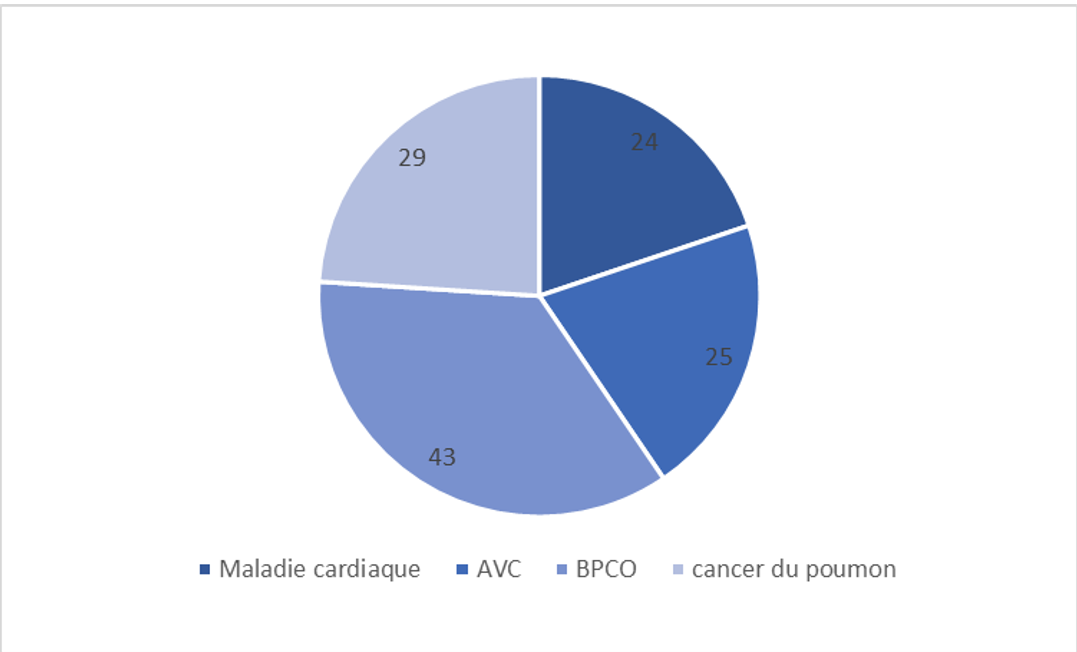
\includegraphics[height=180pt]{images/circle.PNG}
        \caption{Répartition des décès causés par la pollution atmosphérique}
 \end{figure}

\subsection{Maladies Cardiaques}
Des études récentes montrent qu’une exposition au long cours à la pollution atmosphérique, même à des niveaux modérés, peut contribuer à l’émergence de pathologies cardiovasculaires chroniques (ex. hypertension artérielle, artériosclérose, insuffisance cardiaque).
Parmi les polluants mis en cause, les particules fines et ultrafines sont considérées comme étant majoritairement responsables des effets sanitaires. Il a été démontré, aussi bien chez le rongeur que chez l’homme, que la matière particulaire pouvait entraîner des effets négatifs sur l’appareil cardiovasculaire. Parmi les événements susceptibles de contribuer à ces effets, figurent l’importance du stress oxydant, lié à la production excessive d’espèces réactives de l’oxygène (EROs), et de la réponse inflammatoire. Même si l’évolution de la réglementation des émissions des véhicules roulants (normes EURO) a conduit, avec la mise en place des filtres à particules, à une réduction importante des particules primaires d’origine automobile dans l’atmosphère, le dioxyde d’azote (NO2) lié à la présence de la catalyse d’oxydation, peut participer aux effets sanitaires.
\cite{Nathalie Ruaux - Santé et pollution atmosphérique-27 Juillet  2017}

\subsection{Accidents vasculaires cérébraux (AVC)}
L'étude publiée en septembre 2023 dans la revue Neurology met en évidence un lien entre l'exposition à court terme à la pollution atmosphérique et les accidents vasculaires cérébraux. Les conclusions de la méta-analyse indiquent que cette exposition peut augmenter le risque d'AVC dans les cinq jours suivant l'exposition. Les chercheurs ont compilé et synthétisé les résultats de 110 études menées en Asie, en Europe, en Amérique du Nord et en Amérique du Sud, portant sur l'incidence des AVC et les concentrations de polluants atmosphériques courants. Cette analyse a montré une corrélation significative entre l'exposition aux polluants atmosphériques et les taux d'AVC, avec une augmentation pouvant atteindre près de 30\% dans les cinq jours suivant l'exposition.

\subsection{Cancer du poumon}
Depuis 2013, les particules de l’air extérieur sont classées comme cancérigènes pour l’Homme par le Centre international de recherche sur le cancer (CIRC) en raison de leur composition et de leur taille, qui leur permettent de pénétrer profondément dans l’organisme. Certains composants de la pollution de l’air extérieur, tels que les gaz d’échappement des moteurs au diésel, le benzène, la matière particulaire et certains hydrocarbures aromatiques polycycliques (HAP), sont identifiés comme des causes de cancer.
Le radon est également une cause significative de cancer du poumon selon l’Organisation mondiale de la santé (OMS), représentant jusqu'à 14 \% des cas selon la concentration moyenne du gaz et la prévalence du tabagisme. Des études ont montré que même de faibles concentrations de radon, présentes habituellement dans les habitations, peuvent contribuer à l'apparition des cancers du poumon. Le risque de cancer du poumon augmente linéairement avec l'augmentation de la concentration moyenne en radon sur le long terme.
\cite{OMS-2023}

\vspace*{1cm}
      Puisque les affections respiratoires représentent une des conséquences sanitaires majeures de la	 pollution atmosphérique, notre étude porte sur les maladies respiratoires, nous proposons d’explorer en détail ce type de maladie. 

\subsection{Les maladies respiratoire}
L’air constitue le premier élément nécessaire à la vie. La respiration est quant à elle, une fonction vitale de l’Homme. Lorsque l’on sait, que nous respirons entre 150 et 750 milliards de nanoparticules chaque jour, Il est impératif de savoir si les lieux que nous fréquentons sont affectés par la pollution atmosphérique, afin de déterminer la pertinence de notre présence en ces lieux.

\subsubsection{Types de maladies respiratoires associées à la pollution atmosphérique :}
\begin{itemize}
        \item Asthme.
        \item Carcinome bronchogénique / bronchique.
        \item Réactions chimiques entre les gaz, pollen, pulvérisation marine.
        \item Maladie pulmonaire obstructive chronique (MPOC). 
    \end{itemize}
\subsubsection{Gaz responsables}
\begin{itemize}
        \item Monoxyde de carbone (CO) 
        \item Le dioxyde d'azote (NO2)
        \item Le dioxyde de soufre(SOx) 
        \item Les particules fines(PM10 et PM2.5)
    \end{itemize}
    
Ces gaz et particules peuvent aggraver les problèmes respiratoires existants et déclencher des maladies respiratoires graves.

\subsubsection{Symptômes}
  \begin{itemize}  
\item Irritation des yeux.
\item Respiration sifflante ou difficulté à respirer.
\item Irritation et inflammation des voies respiratoires (toux).
\item Augmentation de l’essoufflement, en particulier durant l’activité physique.
\item Aggravation de l'asthme et des troubles cardiaques et pulmonaires existants.
\end{itemize}

Des agents biologiques, tels que les pollens et moisissures, peuvent également être responsables d’effets sur la santé. Par ailleurs, il existe plusieurs types d’interactions entre polluants de l’air et pollens puisque certains polluants chimiques de l’air peuvent favoriser la réaction allergique en abaissant le seuil de réactivité bronchique et/ou en accentuant l’irritation des muqueuses nasales ou oculaires et peuvent également agir sur les grains de pollen, par exemple via la déformation ou la rupture de la paroi du grain de pollen, qui leur permettrait ensuite de pénétrer plus profondément dans le système respiratoire que les grains de pollen entiers.
\cite{} 

\section{Quelques méthodes et technologies}
La détection de la pollution de l'air a fait l'objet de nombreux travaux de recherche. Dans ce qui suit, nous présentons une synthèse de quelques-uns :

[M Rogulski and A Badyda,Current trends in network based air quality monitoring systems, 2019],les auteurs examinent les enjeux environnementaux liés aux technologies employées dans les réseaux de surveillance de la qualité de l'air. Ils se concentrent particulièrement sur les réseaux de mesures de la qualité de l’air, soulignant l'importance cruciale de ce critère dans le déploiement des systèmes IoT. Les auteurs abordent des aspects tels que le coût des capteurs, les types de réseaux et les technologies de transmission couramment utilisées. 
\vspace*{0.5cm}

[M. Sathya et al.,Internet of things (IoT) based health monitoring system and challenges,2018], Dans cet article, l’auteur a utilisé les technologies Peer-to-Peer (P2P) et un système IoT basé sur le cloud qui sont combinées dans un système médical appelé "smart box" pour maintenir les patients sous contrôle. Il a utilisé un système qui se compose de quatre couches de protocole : la couche physique, la couche réseau, la couche middleware et la couche d'application. Il a également utilisé des capteurs portables placés en contact avec la peau sur plusieurs parties du corps capables de mesurer plusieurs facteurs. Ensuite, un petit matériel capable de prétraiter les données acquises est utilisé, et les données sont transmises au cloud pour le stockage d’une manière qui présente une basse consommation d'énergie.
Un critère a été abordé sur la sécurité lors de la transmission vers le stockage des données. Pour une surveillance efficace de la santé, des techniques de visualisation et des algorithmes d'apprentissage automatique ont été abordés pour l’analyse.

\vspace*{0.5cm}

[Vimal Kumar M N et al.,Smart Air Quality Monitoring System in Realtime using IoT,Avril 2021], L'article propose un système de surveillance intelligente de la qualité de l'air en temps réel à l'aide de l'Internet des objets (IoT) pour surveiller les niveaux de pollution de l'air. L'article met en évidence des détecteurs de bruit et d'autres dispositifs permettant une surveillance à distance utilisée pour détecter divers polluants atmosphériques, il mentionne les capteurs utilisés et les technologies de transmission, Il aborde également d'autres facteurs de pollution comme l'humidité.

\vspace*{0.5cm}

[D.N. Paithankar et al.,Framework for implementing air quality monitoring system using LPWA-based IoT technique,2023], L'article décrit un cadre pour la mise en place d'un système de surveillance de la qualité de l'air utilisant la technique IoT. Ils ont utilisé une architecture innovante centrée sur 3 couches. La première est la couche de détection, utilisant des nœuds de surveillance qui surveillent la qualité de l'air et sont alimentés par un système de batterie solaire longue durée. Ensuite, la couche réseau utilise un réseau LPWA basé sur IEEE 802.15.4k pour connecter les nœuds de surveillance au Point d'Accès. Enfin, la couche d'application est composée de deux parties du système : le cloud IoT et les applications client.
Il décrit aussi le matériel et la mise en œuvre logicielle, ainsi que les résultats expérimentaux et l'analyse démontrant l'efficacité du système dans la surveillance de la qualité de l'air.

\vspace*{0.5cm}

[Silvia Liberata and G. R. Sinha ,Advances in Smart Environment Monitoring Systems Using IoT and Sensors,2020] ,L'article examine en détail les différentes méthodes et technologies utilisées pour surveiller l'environnement, en mettant l'accent sur la qualité de l'air et de l'eau. Il met en évidence l'utilisation de capteurs hétérogènes déployés dans des réseaux mobiles et fixes. De plus, il souligne l'importance croissante des dispositifs IoT dans la collecte et l'analyse des données de qualité de l'air, permettant une surveillance en temps réel et une communication efficace entre les différents composants du système. L'article met également en avant l'adoption de technologies émergentes telles que l'intelligence artificielle (IA) et l'apprentissage automatique pour analyser les données des capteurs et prédire la qualité de l'air.

\section{Synthèse et discussion}
La détection de la pollution de l'air grâce à l'utilisation de capteurs et de l'Internet des Objets (IoT) est une approche innovante qui suscite un intérêt croissant en raison de ses implications importantes pour la santé publique et l'environnement. Cette convergence technologique permet de surveiller la qualité de l'air en temps réel et d'identifier les sources de pollution de manière plus précise et efficace.
Cette étude couvre différentes phases : la collecte, la transmission, le stockage, l'analyse et la visualisation des données. L'importance de la sécurité dans ce contexte est primordiale pour protéger l'intégrité des données et garantir la confidentialité des informations collectées, tout en optimisant les coûts, qui est un aspect crucial de cette étude.
En utilisant des technologies efficaces et en optimisant les différentes phases du processus, nous avons dressé dans le tableau suivant une comparaison des différents travaux de recherche sur les techniques utilisées pour la détection de la qualité de l'air, notamment en ce qui concerne l'acquisition, l'analyse et la visualisation des données. 

\vspace*{2cm}
\begin{table}
  \centering
  \begin{tabular}{p{0.9cm}|p{1.2cm}|p{1.2cm}|p{0.75cm}|c|p{0.9cm}|p{0.75cm}|p{0.90cm}|p{0.5cm}|p{0.5cm}|p{0.5cm}|p{1cm}|p{0.7cm}|p{2cm}}
   \hline
   \multirow{2}{*}{\textbf{Article}} & \multicolumn{2}{|c|}{\textbf{Collect}} & \multicolumn{2}{c|}{\textbf{Transmission}} & \multicolumn{2}{c|}{\textbf{Stockage}} & \multicolumn{2}{c|}{\textbf{Type réseau}} & \multicolumn{2}{c|}{\textbf{Analyse}} & \multicolumn{2}{c|}{\textbf{Intégration GIS}} & \multicolumn{1}{c}{\multirow{1}{*}{\textbf{Domaine}}} \\
   & Capteur intelligent & Capteur non intelligent & LoRa & WiFi & Strea- ming data & Batch data & Mobile & Fixe & ML & DL & Mobile GIS & Web GIS & 
 \textbf{d'application} \\

   \hline
   [1] &  & \checkmark & & \checkmark &\checkmark &  &\checkmark &\checkmark & &  & \checkmark &\checkmark & Environnement et santé publique \\
   \hline
   [2] & & \checkmark &  &\checkmark & \checkmark & \checkmark & \checkmark &  & \checkmark & &\checkmark & & Santé \\
   \hline
   [3] &  & \checkmark &  & \checkmark & \checkmark &\checkmark & \checkmark & \checkmark & & &\checkmark & & Environnement et santé publique. \\
   \hline
   [4] &  & \checkmark &  & & \checkmark &\checkmark & &\checkmark & & &\checkmark &\checkmark & Santé \\
   \hline
   [5] & \checkmark & & \checkmark & &\checkmark & &\checkmark &\checkmark & \checkmark &\checkmark & & &Environnement ,L’agriculture   \\
   \hline
  \end{tabular}
 \caption{Tableau avec colonne "Domaine d'application" compacte}
\label{tab:compact}
\end{table} 
\vspace*{0.5cm}

À la suite de cette analyse sur la détection de la pollution de l'air dans le contexte de l'IoT, il est manifeste que cette approche novatrice ouvre des perspectives cruciales pour la surveillance en temps réel de la qualité de l'air. Cependant, il est important de noter que malgré les progrès significatifs dans ce domaine, certaines applications, notamment dans le secteur de la santé, restent encore peu explorées par les chercheurs.
La majorité des articles couvrent les étapes d'acquisition et d'analyse des données,la collecte, la transmission et le stockage des données sont également des aspects abordés, bien que certains articles ne mentionnent pas explicitement ces phases.La visualisation des données semble être moins abordée, avec seulement quelques articles l'incluant dans leurs travaux.
Ces informations soulignent l'importance accordée à la collecte et à l'analyse des données dans le domaine de la détection de la pollution de l'air à travers les systèmes IoT. Cependant, il reste des aspects à explorer plus en détail, notamment en ce qui concerne la visualisation des données pour une meilleure compréhension et prise de décision.
tant que 
En se basant sur ces travaux antérieurs, notre étude s'appuie sur des fondements solides pour explorer les technologies utilisées.

\section{Conclusion}
Dans ce chapitre, nous avons exposé des définitions détaillées sur la pollution en général. Puisque notre étude concerne la pollution de l'air, nous avons abordé les différents polluants atmosphériques ainsi que les informations spécifiques à chaque polluant. Enfin, nous avons examiné les risques de la pollution de l'air sur la santé humaine. Étant donné que l'évaluation de la pollution repose sur les capteurs IoT, cela nous oriente vers le développement d'un système IoT pour l'évaluation de la qualité de l'air dans une région donnée. 


\chapter{IOT et GIS-IOT}
\newpage
\section{Introduction}
L'Internet des Objets (IdO) apporte des avancées significatives dans des domaines clés comme la santé et le transport. Son association avec les Systèmes d'Information Géographique (SIG) attire beaucoup d'attention, car la localisation géographique joue un rôle crucial dans nos activités quotidiennes. Les SIG, reconnus pour leur capacité à traiter les données spatiales de manière exhaustive, sont essentiels pour comprendre et représenter les entités en fonction de leur position et de leur forme. D'un autre côté, l'IdO facilite la communication et l'échange de données entre divers appareils, formant ainsi un réseau étendu d'objets interconnectés.

\vspace*{0.3cm}

L’ intégration entre les SIG et l'IdO ouvre de nouvelles perspectives dans la collecte, l'analyse et la visualisation des données spatiales en temps réel. Elle permet également l'intégration harmonieuse d'appareils connectés dans un réseau géospatial intelligent, favorisant une prise de décision éclairée et l'émergence de solutions innovantes dans des domaines tels que la gestion urbaine, la surveillance environnementale et la logistique.

\vspace*{0.3cm}
Dans ce chapitre, nous allons explorer les concepts de l'Internet des Objets (IdO) et ses architectures, ainsi que la notion des Systèmes d'Information Géographique (SIG). Ensuite, nous discuterons de l'architecture GIS-IoT qui combine ces deux domaines. Nous examinerons également les différentes technologies utilisées pour chaque phase de l'architecture IdO. Par la suite, nous aborderons le rôle des Big Data dans le contexte de l'IdO, et enfin, nous traiterons des technologies d'analyse dans le contexte des Big Data.

\section{Systèmes d'Information Géographique (SIG)}
Dans la littérature, on rencontre différentes définitions des SIGs, nous en avons choisi de 
retenir celles-ci.

\enquote {Le Système d'Information Géographique (SIG) est un outil informatique qui permet de collecter, stocker, gérer, analyser et représenter des données géo-référencées pour faciliter la prise de décision et résoudre des problèmes liés à l'espace et à la localisation.}\cite{Ershad Ali ,2020}
\vspace*{0.2cm}

\enquote{Le Système d'Information Géographique (SIG) est un ensemble puissant d'outils qui traitent la capture de données géospatiales, la gestion de ces données dans une base de données, l'analyse et la reconnaissance de motifs, et enfin la visualisation de l'information.  En tant que principale caractéristique du SIG, il est capable de décrire chaque entité par des données spatiales basées sur son emplacement et sa forme. Les fonctionnalités du SIG couvrent un large éventail d'applications. Pour être plus spécifique, ce cadre est utile pour traiter les requêtes des utilisateurs, qui peuvent être divisées en trois types : factuelles, graphiques et spatiales. Les quatre capacités du SIG (Capture, Gestion, Analyse, Visualisation) sont impliquées dans le processus de réponse aux requêtes des utilisateurs. Cela signifie qu'après la capture des données, selon le type de requêtes des utilisateurs, le SIG peut effectuer des analyses pour fournir des résultats appropriés. Présenter les capacités de stockage de tous les réservoirs situés dans des parcelles d'une ville, visualiser la distribution des centres commerciaux au centre-ville, localiser les parcelles à moins de 2 km d'une centrale électrique sont respectivement quelques exemples de requêtes factuelles, graphiques et spatiales.
}\cite{Jalal Safari Bazargani and al.,2021}

\section{Internet des objets (IOT)}
\subsection{Définitions}
Avant de définir les concepts d’IdO (IoT), il est important de définir l’objet connecté qui est un dispositif dont la finalité première n’est pas d’être un système informatique ni une interface d’accès au web, exemple, un objet tel qu’une machine à café ou une serrure était conçue sans intégration de systèmes informatiques ni connexion à Internet. L’intégration d’une connexion Internet a un OC permet de l’enrichir en terme de fonctionnalité, d’interaction avec son environnement, il devient un OC Enrichi (OCE), par exemple, l’intégration d’une connexion internet à la machine à café la rendant accessible à distance.

Selon \cite{Çetin Önder İncekara,2023} L'Internet des Objets a été défini comme suit : \enquote{L'Internet des Objets est un système qui interconnecte un réseau d'objets physiques tels que des capteurs, des dispositifs informatiques et des logiciels pour transférer des données vers d'autres systèmes sans aucune interférence de l'interaction humaine à humaine ou humaine à ordinateur, c'est-à-dire les maisons intelligentes. La croissance de l'industrie des télécommunications nous offre de nouvelles offres de connectivité comme le service 6G qui sera bientôt connecté.

Les appareils pouvant se connecter à l'IdO vont des appareils ménagers ordinaires aux grands équipements industriels. Il est utilisé pour le calcul et pour minimiser l'intervention humaine. Avec l'IdO, les gens collectent et partagent automatiquement les données pour les aligner avec leur processus quotidien avec les machines ou leur mode de vie.

L'Internet des Objets peut être défini comme un réseau qui permet aux objets autour de nous de s'interconnecter et de communiquer entre eux. Les objets autour de nous sont intelligents : montre intelligente, télévision intelligente, téléphone intelligent, et plus encore. L'avenir de l'IdO est vaste et l'avenir reposera sur les technologies de l'IdO.}

\enquote{ L’IoT un système d'appareils, de capteurs et de machines numériques interconnectés qui peuvent communiquer et partager des données sur un réseau sans nécessiter d'interaction humaine.
Il offre un potentiel unique pour collecter des données afin de les utiliser dans différentes applications. Le développement de ce domaine dépend des appareils ou capteurs IoT qui sont considérés comme son système nerveux. Les capteurs IoT jouent un rôle primordial dans le fonctionnement de l’IoT. Ils détectent les changements d’un environnement, mesurent, collectent et transforment ses données pour pouvoir ensuite être exploitées par les analystes des données.}\cite{Hesna Mrabti-Proposition d’une annotation sémantique des données issues d’IoT-juin 2022}

\subsection{Architecture IOT}
L'architecture de l'Internet des Objets (IoT) comprend plusieurs éléments de systèmes connectés pour assurer la collecte, le stockage et le traitement des données générées par les capteurs dans des entrepôts de données volumineuses (big data), ainsi que l'exécution des commandes par les actionneurs des objets via une application utilisateur.

C'est un cadre qui définit les composants physiques, l'organisation fonctionnelle, la configuration du réseau, les procédures opérationnelles et les formats de données à utiliser.

Cependant, il n'existe pas de modèle d'architecture standard unique pour l'IoT en raison de la diversité des technologies impliquées. Cela signifie qu'il n'y a pas de modèle simple qui puisse être appliqué à toutes les implémentations possibles.
\vspace*{0.2cm}

La figure suivante montre le format le plus basique et le plus largement accepté est une architecture IoT à quatre couches.\cite{Web 6 : iotindustriel.com}
  \begin{figure}[h]
        \centering
        \fbox{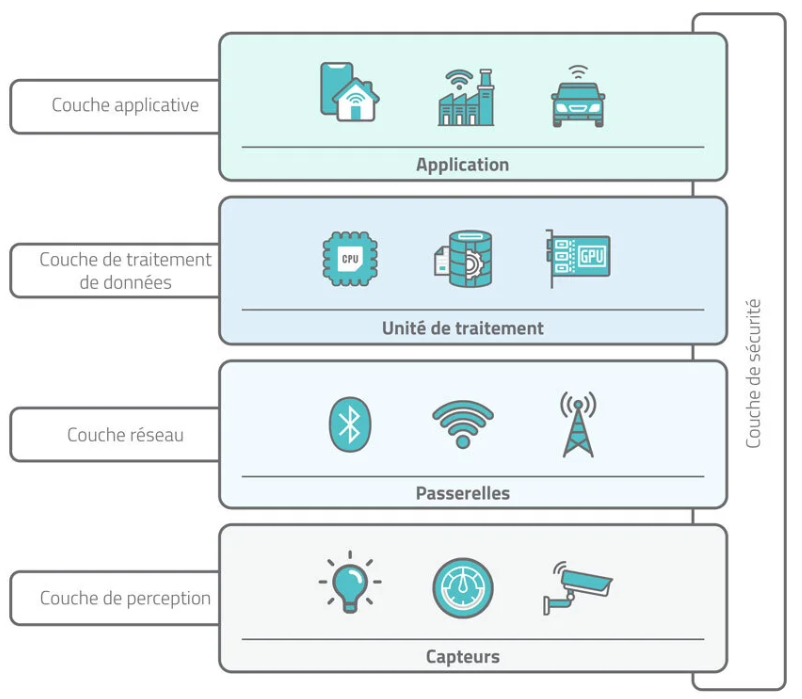
\includegraphics[height=300pt,width=300pt]{images/iot-archi}}
        \caption{Architecture IOT \cite{Web 6 : iotindustriel.com}}
        \label{b}
    \end{figure}
\vspace*{0.5cm}

\begin{itemize}
\item {\large\textbf{Couche perception}}  \\

Cette couche est chargée de la conversion des signaux analogiques en données numériques et vice versa. Dans les premières étapes de tout système IoT, une diversité d'objets joue le rôle de lien entre le monde réel et le monde numérique. Ces objets varient en forme et en taille, allant des minuscules puces de silicium aux gros véhicules. Ils se répartissent en différentes catégories selon leurs fonctions :
\begin{enumerate}
\item \textbf{Capteurs} \\
Un capteur IoT, qu'il s'agisse d'un capteur d'objet connecté ou d'un capteur classique, est conçu pour détecter différents types d'énergie tels que les gaz, la lumière, la force, etc., et les convertir en données numériques. Ces capteurs, qui peuvent prendre la forme de sondes, de jauges, de compteurs et autres dispositifs, recueillent des informations sur des paramètres physiques comme la température ou l'humidité. Ils transforment ensuite ces données en signaux électriques qu'ils envoient au système IoT. En général, les capteurs IoT sont de petite taille et consomment peu d'énergie. \cite{Web 6 : iotindustriel.com} \\
 
  \begin{figure}[h]
        \centering
        \fbox{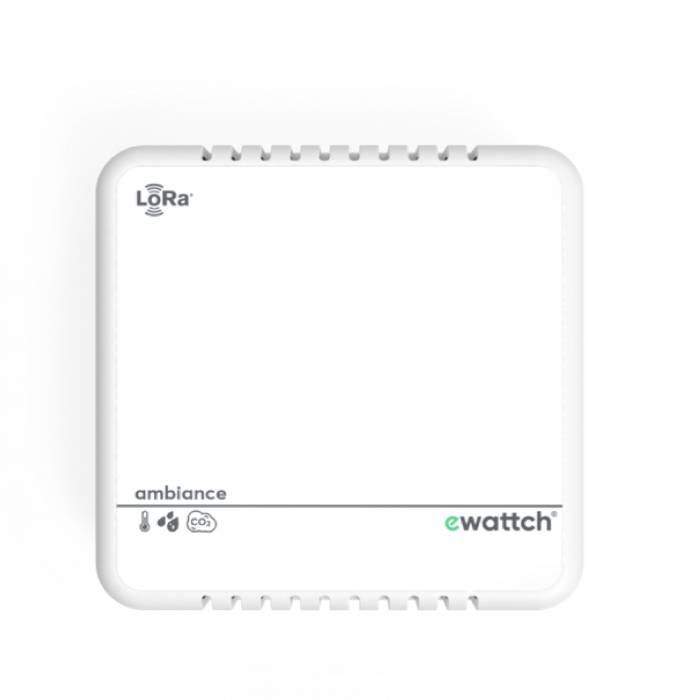
\includegraphics[height=250pt,width=250pt]{images/capteur}}
        \caption{Capteur IoT LoRaWAN \cite{Web 7 :www.ip-systemes.com}}
        \label{b}
    \end{figure}
\item \textbf{Actionneurs} \\
Ils traduisent les signaux électriques du système IoT en actions physiques, utilisés dans les contrôleurs de moteur, les lasers, les bras robotiques, etc.\\

\item \textbf{Machines et dispositifs} \\
Connectés à des capteurs et des actionneurs ou comme étant des parties intégrantes.
\end{enumerate} 
\vspace*{0.5cm}
\item {\large\textbf{Couche réseau}} \\

Cette couche agit comme les nerfs humains,elle est responsable de la connexion au système de traitement pour transmettre les informations recueillies par les appareils capteurs. Une large gamme de réseaux de communication comme les réseaux câblés ou sans fil, Internet, etc., peut être intégrée à la couche perception.

Parmi les moyens de communication utilisés dans cette couche, on retrouve les suivants \cite{Bilal Benamrouche,2018} :
\begin{enumerate}
\item \textbf{Wi-Fi} \\
La norme de réseau sans fil IEEE 802.11, également connue sous le nom de Wi-Fi (Wireless Fidelity), est largement utilisée pour les communications entre ordinateurs, dispositifs mobiles tels que les téléphones portables, et Internet. Il permet de gérer de grandes quantités de données grâce à un haut débit de transfert.\\
\item \textbf{ZigBee} \\
une norme adaptée aux applications nécessitant une communication sans fil à faible consommation d'énergie et à bas débit  également appelés WPAN, offrant une portée étendue et des options de configuration réseau variées.

\item \textbf{SIGFOX} \\
SIGFOX est une entreprise pionnière dans le domaine des réseaux LPWAN (Low-Power Wide-Area Network) dédiés à l'Internet des Objets (IoT). 
La technologie SIGFOX repose sur une modulation ultra-étroite (UNB), qui permet une utilisation efficace et optimisée du spectre radioélectrique. Cette modulation est adaptée aux besoins de l'IoT, car elle permet une transmission de données à faible puissance sur de longues distances, avec une consommation d'énergie réduite. \\

\item \textbf{LoRaWAN} \\
 C'est un protocole de réseau et une architecture de communication ouverts, conçus pour les objets connectés et les appareils à faible consommation d'énergie, tels que les capteurs et les actionneurs, dans le contexte de l'Internet des objets (IoT). \\
LoRaWAN repose sur deux couches distinctes : \\
\textbf {Couche physique LoRa (LoRa PHY) :} Utilise la modulation de radio LoRa, basée sur la technique de modulation de spectre étalé par étalement de fréquence (CSS - Chirp Spread Spectrum). Cette couche offre une portée de communication étendue et une consommation d'énergie réduite, adaptée aux appareils IoT à faible consommation d'énergie.\\
\textbf{Protocole de couche MAC LoRaWan : } Il fournit un accès au réseau LoRa. LoRaWAN est un protocole ouvert standardisé, permettant la communication entre les appareils finaux (capteurs, actionneurs, etc.) et les passerelles LoRaWAN, ainsi que la gestion du réseau et des données. 
            [Jetmir Haxhibeqiri et al..,2018]
\end{enumerate}
\vspace*{0.5cm}
\item {\large\textbf{Couche de traitement de données}} \\

Cette couche est conçue pour stocker, analyser et traiter les informations reçues de la couche Perception via la couche Réseau. Un accès direct à une base de données pour stocker les informations est fourni en utilisant des technologies comme le cloud et le fog computing.
\vspace*{0.5cm}
\item {\large\textbf{Couche applicative}} \\

 La couche d'application joue le rôle d'interface entre le système et l'utilisateur. En raison des données traitées et de l'objectif du système conçu, cette couche est responsable de fournir l'application appropriée à l'utilisateur.

\end{itemize}
 \vspace*{0.5cm}  

\subsection{Architecture GIS-IOT}
L'intégration du SIG dans les systèmes IoT élargit les dimensions et les possibilités des applications IoT, car le SIG peut gérer à la fois les données spatiales et attributives collectées par les capteurs. \\
  \begin{figure}[h]
        \centering
        \fbox{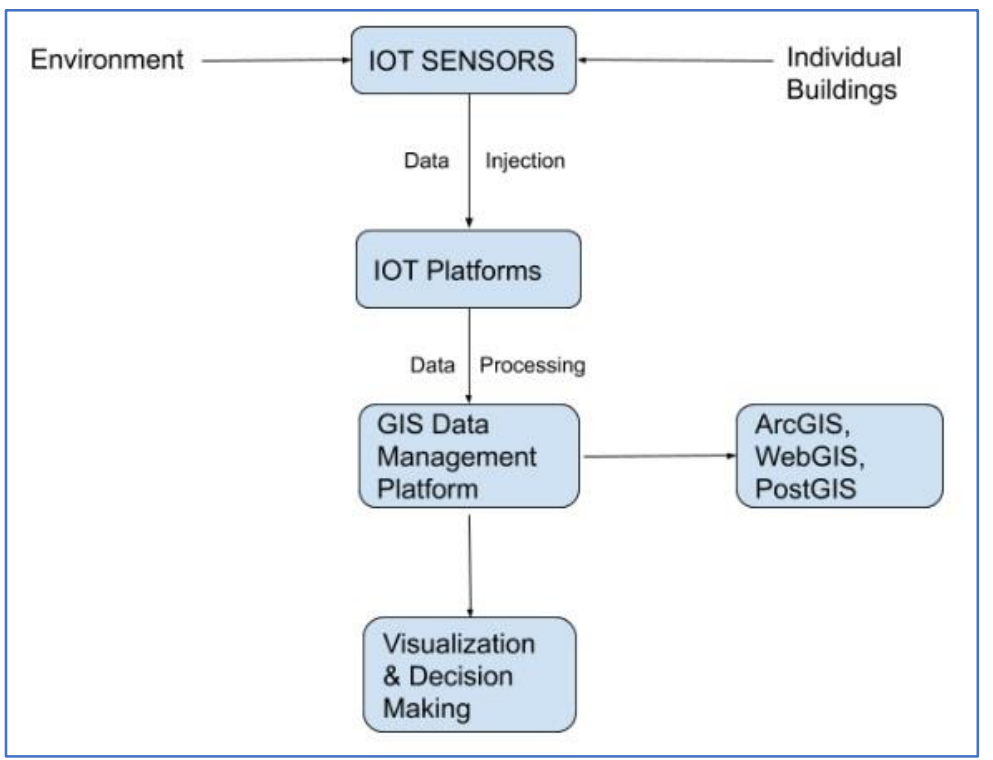
\includegraphics[height=300pt,width=300pt]{images/gis-iot}}
        \caption{ Architecture système de couplage IoT et Organigramme SIG \cite{[Çetin Önder İncekara et al.,Internet of Things (IoT) in GIS, 5 mars 2023}}
        \label{b}
    \end{figure}

L'injection de données stocke les informations collectées sur les plates-formes IoT, telles que les technologies qui gèrent, fournissent et se connectent au monde IoT. L'étape suivante est le traitement des données, où les données collectées à partir de l'IoT sont utilisées dans les plateformes SIG. Les données collectées sont destinées à la manipulation, au stockage et à l'analyse par les applications WebGIS, PostGIS et ArcGIS. La visualisation et la prise de décision consistent à utiliser toutes les données dans les couches cartographiques. À partir des données identifiées, les gens peuvent visualiser l'environnement et les lieux. \\

L'organigramme de la figure suivante présente l'architecture système de couplage IoT et SIG. \\

\newpage
\vspace*{1cm}
La convergence des technologies des Systèmes d'Information Géographique (SIG) et de l'Internet des Objets (IoT) ouvre de nouvelles perspectives passionnantes dans la gestion des données spatiales et la connectivité des objets. En intégrant les capteurs IoT dans l'architecture des SIG, nous avons désormais la capacité de collecter en temps réel une grande quantité de données sur les objets et les événements dans l'environnement physique. Cette approche permet non seulement de visualiser et d'analyser spatialement ces données, mais elle ouvre également la porte à l'exploration du concept du Big Data. \\

La prochaine section sera donc dédiée à la mise en œuvre pratique des concepts et des méthodologies du Big Data.

\vspace*{1cm}
\section{BIG-GÉO Data dans context IOT}
Le Big Geo Data dans le contexte de l'IoT fait référence à la gestion et à l'analyse de vastes ensembles de données géospatiales générées par les objets connectés. Ces données comprennent des informations sur la localisation, les mouvements, les interactions et d'autres aspects géographiques des objets et des événements capturés par les capteurs IoT. \\

Selon \cite{Marina Ptiček and Boris Vrdoljak , 2017} , Le Big Data a été défini comme \enquote{Le terme "big data" fait référence à des ensembles de données vastes et complexes qui dépassent les capacités des méthodes et des outils traditionnels de traitement des données. Il englobe de grandes quantités de données générées à partir de diverses sources, notamment les transactions commerciales, les interactions sur les médias sociaux, les données des capteurs, et bien plus encore. Ce terme décrit les types de données nouvellement émergés, qui sont généralement caractérisés par les 4V, mais aussi récemment par les 7V : \\
\begin{itemize}
\item Volume : les quantités de données sont vastes.
\item Variété : il existe un grand nombre de formats de données et des niveaux variables de structuration des données.
\item Vélocité : les big data arrivent à grande vitesse et le traitement en temps réel est crucial.
\item Vérité : les données peuvent être incorrectes ou inconsistantes dans une certaine mesure.
\item Variabilité : les mêmes données peuvent être interprétées de différentes manières et donc produire des résultats différents.
\item Valeur : l'utilité réelle des informations extraites n'est pas garantie.
\item Visualisation : les données doivent être visualisées pour en améliorer la compréhension.
\end{itemize}}

\subsection{Architectures Big Data}
Entrez dans l'ère de la révolution des données, où les structures Big Data ont progressé pour répondre aux besoins croissants de stockage, de traitement et d'analyse des informations à grande échelle. Parmi ces structures, deux concepts clés se distinguent : les structures Lambda et Kappa.

\begin{itemize}
\item  {\large\textbf{Lamda}} \\
L’architecture lambda a été proposée pour la première fois par \textit{Nathan Marz}, dans cette architecture les données sont stockées dans une couche de persistance comme HDFS, d'où elles sont collectées et traitées périodiquement par la couche batch. En parallèle, la couche de vitesse gère la partie des données qui n'a pas encore été traitée par la couche batch, tandis que la couche de service fusionne les sorties de la couche batch et de la couche de vitesse pour les consolider. \cite{Wingerath et al.,Real-time streaming analytics for Big Data, 2016}  \\
Dans le schéma ci-dessus, vous pouvez observer les principaux éléments de l'Architecture Lambda :
\vspace*{1cm}
  \begin{figure}[h]
        \centering
        \fbox{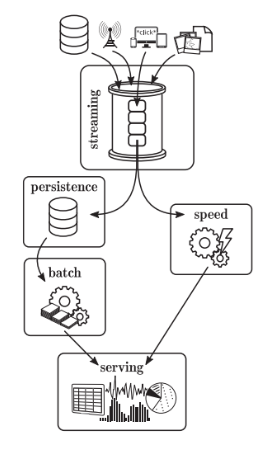
\includegraphics[height=300pt,width=200pt]{images/lamda}}
        \caption{ Architecture lamda \cite{[Wingerath et al.,2016}}
        \label{b}
    \end{figure}
\newpage
\textbf{Couche de Persistance (HDFS) :} Cette phase est responsable de stocker les données, généralement dans un système comme HDFS, à partir duquel elles sont traitées périodiquement par la couche batch.\\

\textbf{Couche Batch :} Cette phase gère le traitement par lots des données. Elle les ingère depuis la couche de persistance selon un calendrier périodique (par exemple, une fois par jour) pour les préparer à l'indexation.\\

\textbf{Couche de Vitesse (Speed Layer) :} Cette phase traite la partie des données qui n'a pas encore été traitée par la couche batch. Elle gère les données en temps réel et contribue à réduire le délai entre l'ajout des données au système et leur disponibilité pour interrogation.\\

\textbf{Couche de Service (Serving Layer) :} Cette phase consolide les sorties de la couche batch et de la couche de vitesse, les fusionnant pour permettre une interrogation cohérente des données par les utilisateurs finaux.\\
\cite{[Wingerath et al.,2016}
\vspace*{1cm}
\item {\large\textbf{ Kappa}} \\

L’architecture kappa a été proposée par \textit{Jay Kreps} comme alternative à l’architecture lambda.
L'idée de base de cette architecture est de ne pas recalculer périodiquement toutes les données dans la couche batch, mais de réaliser tous les calculs dans le système de traitement en continu seul et de ne réaliser une recomputation que lorsque la logique métier change en rejouant les données historiques.\cite{Wingerath et al.,2016} \\
Nous présentons ci-dessus l'architecture Kappa

 \begin{figure}[h]
        \centering
        \fbox{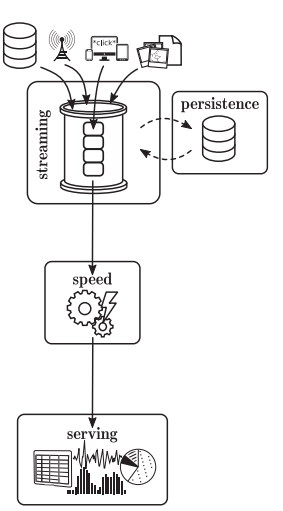
\includegraphics[height=300pt,width=200pt]{images/kafka}}
        \caption{ Architecture Kappa \cite{[Wingerath et al.,2016}}
        \label{b}
    \end{figure}


\end{itemize}
\newpage
\subsection{Approches de Big Data}
Dans le domaine de la gestion des données pour stocker et organiser des informations, on a trois concepts qui sont utilisés : \\
\begin{itemize}
\item Base de données NoSQL database.
\item Un entrepôt de données (ou "datawarehouse" en anglais).
\item Un lac de données (ou "data lake" en anglais). \\
\end{itemize} 
Ils diffèrent dans leurs approches et leurs fonctionnalités principales.

\subsubsection{NoSQL (Not Only SQL)}
NoSQL est présenté comme une tendance souvent mal interprétée. Contrairement à ce que son nom pourrait laisser penser, NoSQL n'exclut pas complètement SQL (Structured Query Language), le langage de requête utilisé dans les bases de données relationnelles. Au lieu de cela, NoSQL implique une extension ou une modification du stockage relationnel traditionnel. Les bases de données NoSQL se caractérisent par leur extensibilité horizontale, leur informatique distribuée et leur meilleure tolérance aux pannes. \\

Il existe quatre principales familles de bases de données NoSQL : 
\begin{itemize}
\item bases de données orientées colonnes
\item bases de données orientées documents
\item stockage clé-valeur
\item bases de données graphiques
\end{itemize}
Pour la recherche en entrepôt de données volumineuses, les familles de bases de données NoSQL les plus importantes sont les bases de données orientées colonnes et les bases de données orientées documents
\cite{Marina Ptiček and Boris Vrdoljak ,2017}

\subsubsection{Entrepôts de données (Data warehousing)}
Un entrepôt de données est un système informatique utilisé pour collecter et gérer d'importantes quantités d'informations provenant de diverses sources au sein d'une entreprise. Ces informations sont généralement organisées de façon à être facilement consultables et analysées pour appuyer les prises de décision et les activités commerciales.\\
La figure suivante montrent l'architecture de l'entrepôts de données :
  \begin{figure}[h]
        \centering
 \fbox{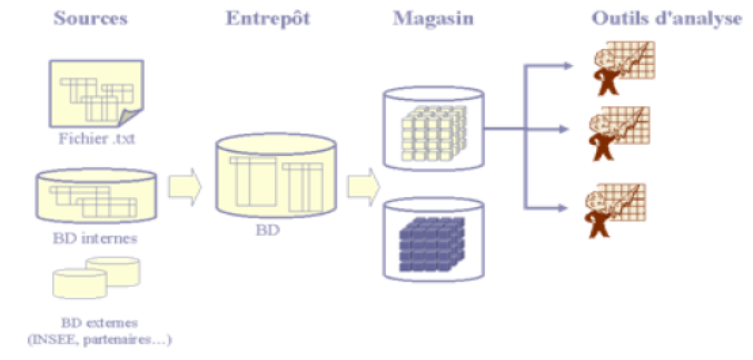
\includegraphics[height=200pt,width=300pt]{images/dataware}}
        \caption{Architecture de l'entrepôts de données \cite{Cécile Favre et al.,January 2013}}
        \label{f}
    \end{figure}
    
    
 \textbf{Magasin de données (Data mart)} 
Un magasin de données détient un sous-ensemble des données d'un entrepôt de données, normalement sous la forme de données résumées, concernant un département ou service particulier ou encore d'une fonction professionnelle précise.

\subsubsection{ Lac de données (Data Lake)}
Le nom du lac de données est inspiré par le lac naturel où tous les organismes et les espèces biologiques ou matériels non-biologiques sont autorisés à y entrer. De la même manière, le lac de données prépare un environnement pour livrer tous types de données (structurées et non structurées) depuis diverses sources. \cite{Marzieh Derakhshannia,2022} \\

L'architecture d'un lac de données est représentée comme illustrée dans la figure suivante :
\begin{figure}[h]
        \centering
 \fbox{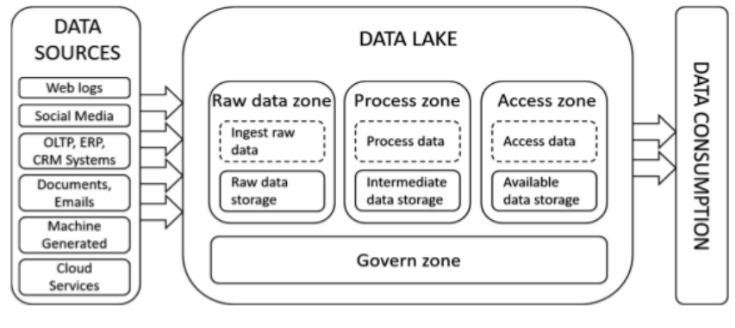
\includegraphics[height=200pt,width=230pt]{images/datalake2}}
        \caption{Architecture de lac de données \cite{Franck Ravat et Yan ZhaoData,2019}}
        \label{f}
    \end{figure} 
    \\
Cette architecture proposée comprend quatre zones essentielles. Chaque zone, à l'exception de la zone de gouvernance, dispose d'une zone de traitement (rectangle en pointillés) et d'une zone de stockage des données qui conserve le résultat des processus (rectangle gris).

\begin{table}[htbp]
\centering

\begin{tabular}{|p{4cm}|p{0.7\textwidth}|}
\hline
\textbf{Zone}             & \textbf{Description} \\
\hline
Zone de données brutes (Raw Data Zone) & Stocke les données dans leurs formats natifs, permettant aux utilisateurs de trouver les versions originales des données pour leurs analyses. \\
\hline
Zone de traitement (Process Zone)& Permet aux utilisateurs de traiter les données (sélection, projection, jointure, agrégation) pour leur analyse. \\
\hline
Zone d'accès  (Acess Zone) & Stocke toutes les données disponibles et prêtes pour les opérations d'analyse, permettant aux utilisateurs d'accéder et de consommer ces données pour différentes analyses. \\
\hline
Zone de gouvernance  (Govern Zone) & S'applique à toutes les autres zones, assurant la sécurité, la qualité et l'accès aux données. \\
\hline
\end{tabular}
\caption{Description des zones d’architecture fonctionnelle de lac de données}
\end{table}
\newpage
\section{Approches d'analyses dans un context Big Data}
L'analyse de données volumineuses, également connue sous le nom de Big Data analytics, consiste à explorer et à extraire des connaissances à partir de grandes quantités de données en utilisant des méthodes avancées, notamment dans le domaine de l'intelligence artificielle. Dans le contexte de l'IoT, nous discuterons des méthodes les plus connues telles que l'apprentissage automatique(Machine learning en anglais) et l'apprentissage profond(Deep Learning en anglais).

\subsection{L'apprentissage automatique (Machine learning)}
  L'apprentissage automatique décrit la capacité des systèmes à apprendre à partir de données d'entraînement spécifiques au problème pour automatiser le processus de construction de modèles analytiques et résoudre des tâches associées. \cite{[Christian Janiesch and al,2021]}
  \subsubsection{Types de machine learning}
  
Il existe quatre méthodologies d'apprentissage fondamentales : l'apprentissage supervisé, l'apprentissage non supervisé, l'apprentissage semi-supervisé et l'apprentissage par renforcement comme le montre la figure suivante
  \begin{figure}[h]
        \centering
    \fbox{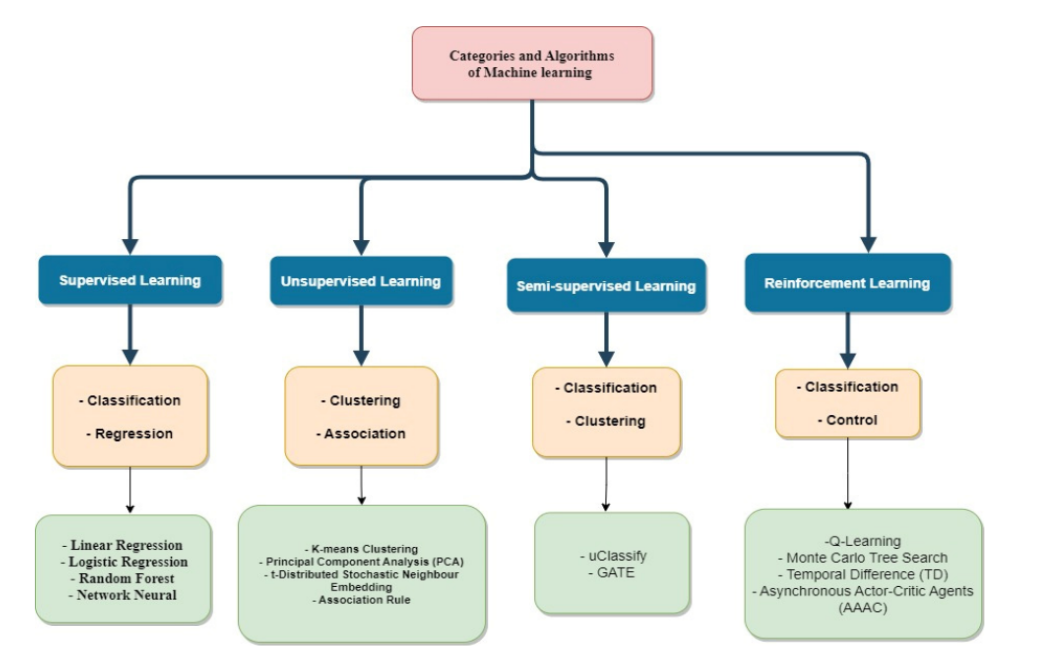
\includegraphics[height=250pt,width=300pt]{images/ml}}
        \caption{les différents types de machine learning.\cite{Mohammad Mustafa Taye,2023}}
        \label{g}
    \end{figure}
 \begin{itemize}
 \item \textbf {L'apprentissage supervisé (Supervised learning) :}  nécessite un ensemble de données d'entraînement qui couvre des exemples pour l'entrée ainsi que des réponses étiquetées ou des valeurs cibles pour la sortie. Il existe deux types de problèmes en Supervised Learning : les problèmes de régression, où une valeur numérique est prédite, et les problèmes de classification, où le résultat de la prédiction est une classe catégorique. \\
 \item \textbf {L'apprentissage non supervisé (Unsupervised Learning) :}  se produit lorsque le système d'apprentissage est censé détecter des motifs sans étiquettes préexistantes ou spécifications. Les données d'entraînement ne consistent qu'en variables x avec pour objectif de trouver des informations structurelles d'intérêt, comme des groupes d'éléments partageant des propriétés communes (clustering) ou des représentations de données projetées d'un espace de grande dimension vers un espace de moindre dimension (réduction de dimension). \\
 \newpage
 \item \textbf {l'apprentissage semi-supervisé (Semi-supervised Learning) :}  utilise à la fois des données étiquetées et non étiquetées pour l'entraînement, réduisant ainsi le besoin en données annotées coûteuses. Il combine des approches supervisées et non supervisées pour détecter des motifs et structures dans les données. Les architectures hybrides fusionnent des composants discriminatifs et génératifs pour des performances améliorées. Cette technique est largement utilisée dans la santé pour l'analyse de la parole et la gestion du contenu numérique, offrant une précision accrue sans nécessiter de grandes quantités de données annotées. \\
 \item \textbf {L'apprentissage par renforcement (Reinforcement Learning) :} décrit l'état actuel du système, spécifie un objectif, fournit une liste d'actions autorisées et de leurs contraintes environnementales, puis laisse le modèle ML expérimenter le processus pour atteindre l'objectif en maximisant une récompense grâce au principe de l'essai-erreur.\cite{Christian Janiesch1 and al,2021}
 \end{itemize}
 
 \subsection{L'apprentissage Profond (Deep learning)}
Le Deep Learning est une branche de l'apprentissage automatique qui vise à représenter le monde par une hiérarchie de concepts détectés automatiquement. Ses modèles, avec leurs nombreuses couches et leur abstraction élevée, offrent des avantages significatifs par rapport aux méthodes traditionnelles. En exploitant de vastes volumes de données, le Deep Learning produit des algorithmes d'apprentissage sophistiqués et précis, ce qui en fait un choix privilégié pour les organisations cherchant des prédictions précises et compétitives à mesure que la quantité de données augmente.\cite{Mohammad Mustafa Taye,2023} \\

Nous allons présenter ci-dessous les différentes architectures de deep learning.

\begin{enumerate}
\item \textbf {Réseau de neurones convolutionnels (CNN) :} Principalement utilisés pour la vision par ordinateur et la reconnaissance vocale, les CNNs sont capables de traiter des ensembles de données avec des relations spatiales comme les données d'images. Ils extraient des caractéristiques hiérarchiques pour reconnaître des objets dans les images. \\

\item \textbf {Réseau de neurones récurrents (RNN) :} Conçus pour les données séquentielles telles que les séries temporelles et le langage naturel, les RNNs utilisent des boucles de rétroaction interne pour apprendre des modèles séquentiels et des dépendances temporelles.\\

\item \textbf {Représentations distribuées :} jouent un rôle essentiel dans l'apprentissage de caractéristiques et la modélisation du langage dans les tâches de traitement du langage naturel. Elles projettent des entités linguistiques dans des espaces sémantiques unifiés sous forme d'embeddings numériques. temporelles.\\

\item \textbf {Autoencodeur :} Fournit une représentation dense des données d'entrée en comprimant l'information dans un espace de dimension réduite, puis en essayant de la reconstruire. Utilisé pour l'apprentissage non supervisé et la réduction de dimensionnalité.\\

\item \textbf {Réseau de neurones antagonistes génératifs (GAN) :} Appartenant à la famille des modèles génératifs, les GANs apprennent une distribution de probabilité sur un ensemble de données d'entraînement pour générer de nouveaux échantillons de manière aléatoire. Ils sont utilisés pour créer de nouveaux contenus et configurations de produits, mais peuvent aussi poser des risques sociétaux s'ils sont utilisés de manière malveillante, notamment pour la création de contenus trompeurs ("deepfake").

\end{enumerate}
\newpage
\begin{itemize}
\item { \large \textbf{Les réseaux de neurons}} \\

Les réseaux de neurones sont des modèles simplifiés des fonctions des neurones dans le cerveau humain, utilisés pour résoudre des problèmes d'apprentissage profond. Ils sont généralement exprimés par une fonction sigmoïde, représentée mathématiquement par :

\[
\centering
f(x) = \frac{1}{1 + e^{-x}}
\]
\begin{itemize}
 \item \textbf{Les réseaux de neurons artificiels (RNA)} \\
Les réseaux neuronaux artificiels (ANN) sont conçus pour simuler le fonctionnement des réseaux de neurones dans le cerveau humain, où les ordinateurs agissent comme des cellules cérébrales interconnectées. Comme différentes parties du cerveau traitent différentes informations de manière hiérarchique ou en couches, les ANN adoptent une approche similaire en couches pour le traitement de l'information et la prise de décision. 
Typiquement, un ANN comporte trois couches de neurones : 
la couche d'entrée pour les données d'entrée.
 la couche cachée pour le traitement des informations.
la couche de sortie pour la décision basée sur les données.
\cite{Tehseen Mazhar and al ,2023} \\
Typiquement, un ANN comporte trois couches de neurones : 

\begin{enumerate}
\item la couche d'entrée pour les données d'entrée.
\item la couche cachée pour le traitement des informations.
\item la couche de sortie pour la décision basée sur les données. \cite{Tehseen Mazhar and al ,2023}
\end{enumerate} 

La figure suivante montre l’architecture des réseaux de neurons artificiels \cite{web 7 : blog.sinatechnologie.com} :
\begin{figure}[h]
        \centering
    \fbox{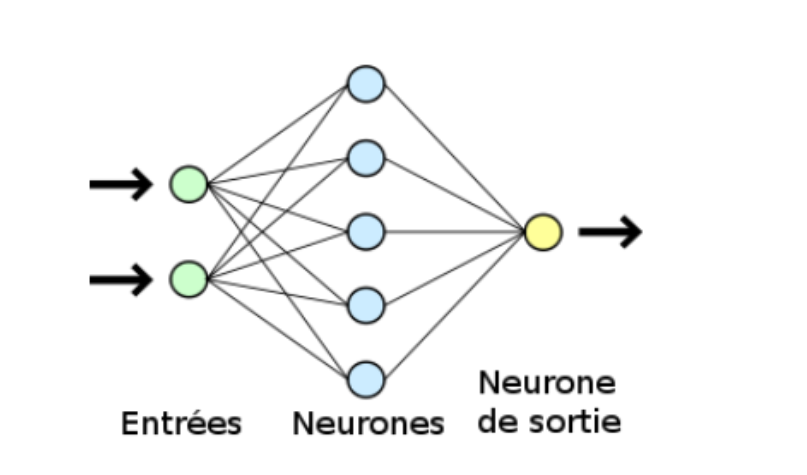
\includegraphics[height=250pt,width=350pt]{images/RN}}
        \caption{Architecture des réseaux de neurons artificiels.\cite{web 7 : blog.sinatechnologie.com} }
        \label{g}
    \end{figure}
\newpage
\item \textbf{ Les réseaux de neurons profonds (DNN)}  \\
Un réseau neuronal profond (DNN) est une extension avancée des réseaux neuronaux artificiels (ANN) avec plusieurs couches entre les entrées et les sorties. Ces réseaux utilisent des manipulations mathématiques complexes pour transformer les entrées en sorties, qu'il s'agisse de relations linéaires ou non linéaires. Les DNN peuvent avoir de nombreuses couches, d'où leur appellation de "réseaux profonds". \\

La figure suivante montre l’architecture du réseau de neuraux profond \cite{web 7 : blog.sinatechnologie.com} :
\begin{figure}[h]
        \centering
    \fbox{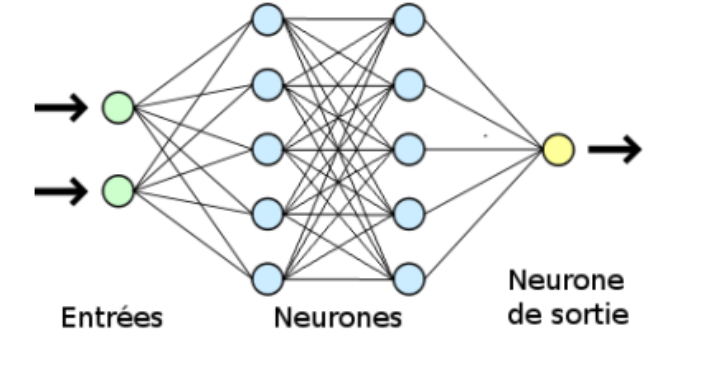
\includegraphics[height=250pt,width=350pt]{images/DNA}}
        \caption{Architecture du réseau de neuron profond  DNN.\cite{web 7 : blog.sinatechnologie.com} }
        \label{g}
    \end{figure}

\end{itemize}

\end{itemize}
\newpage
\section{Modélisation des données}
\subsection{Diagramme de classe}
Il représente les classes intervenant dans le système. Le diagramme de classe est une représentation statique des éléments qui compose un système et de leurs relations.Chaque application serra une instance des différents classe qui le composent , à ce titre il faudra bien gardé à l'esprit qu'une classe est un modèle , et l'objet ça réalisation.
\\
    \begin{figure}[h]
        \centering
           % \fbox{\includegraphics[height=480pt,width=\linewidth]{images/classs.jpg}}
        \caption{Diagramme de classe}
    \end{figure}

\textbf{NB:} une description détaillée des classes et des tables de la base de données est présentée dans les annexes \ref{a1} à partir de la page \pageref{a1} et \ref{a2} à partir de la page \pageref{a2}.
\newpage
\subsection{Modèle Relationnel de données}

\begin{description}
\vspace*{1cm}
    \item \large{\textbf{Employé}} ( \ul{id\_employe} , nom\_employe , prenom\_employe , date\_naiss , lieu\_naiss, adresse , tel , email , grade , id\_service* )\\
    \item \textbf{Compte} ( \ul{id\_compte} , nom\_utilisateur , mot\_de\_passe , id\_employe* )\\
    \item \textbf{Direction} ( \ul{id\_direction} , nom\_direction )\\
    \item \textbf{Service} ( \ul{id\_service} , nom\_service , id\_direction* )\\
    \item \textbf{Projet} ( \ul{code\_projet} , description , id\_direction* )\\
    \item \textbf{Chantier} ( \ul{code\_chantier} , localisation , remarque , code\_projet* )\\
    \item \textbf{Dem\_appro} ( \ul{ref\_appro} , type\_prestation , design\_prestation , montant\_max,montant\_min, date\_insertion , dernier\_delai , code\_chantier*, id\_employe* )\\
    \item \textbf{Affectation} ( \ul{ref\_appro* , id\_employe*} , date\_affectation , statut )\\
    \item \textbf{Fournisseur} ( \ul{id\_fournisseur} , nom\_fournisseur , domaine , adresse , telephone, email , fax , contact )\\
    \item \textbf{Operation} ( \ul{ref\_operation} , type\_operation , motif , comission , heur\_ouverture, nbr\_retraits , statut\_operation, ref\_appro* )\\
    \item \textbf{Contrat} ( \ul{ref\_contrat} , design\_contrat , montant , device , date\_debut , id\_fournisseur*, ref\_operation* )\\
    \item \textbf{Reg\_retrait} ( \ul{ref\_operation* , id\_fournisseur*} , dateTime\_retrait )\\
\end{description}
\vspace{0.7cm}
\section{Conclusion}
A cette phase du projet nous avons pus définir les différents acteurs et toute les fonctionnalités de notre système.\\
Les diagrammes de cas d’utilisations, nous on permis de lister les tâches établis et cela on adoptant le point de vue des acteurs, tandis qu'on a réussi grâce aux diagrammes de séquence  de représenter les interactions entre les acteurs et le système selon un ordre chronologique.Et nous avons clôturé notre phase d'analyse et de conception par la représentation du diagramme de classe de notre base de données et le passage vers le modèle relationnel.\\
L'étape suivante présente brièvement notre solution informatique et les différentes technologies utilisés.

%Chapter Three Réalisation
\chapter{Réalisation}
\newpage
\section{Introduction}
Après avoir finalisé l’étape de conception, nous consacrons ce chapitre à la réalisation.\\
Le problème a été profondément analysé, ce qui va nous permettre alors d’entreprendre le développement de l’application, ayant comme objectif d’aboutir à un produit final, exploitable par les différents utilisateurs.\\
Nous allons d’abord présenter l’environnement de développement ainsi que les outils et les logiciels utilisés, et quelques interfaces graphiques de l’application réalisée.\\
\section{Présentation de l’architecture 3-tiers}
Une application Web possède souvent une architecture 3-tiers.\\
\begin{description}
    \item{\textbf{La couche DAO :}} " Data Access Object " s'occupe de l'accès aux données, le plus souvent des données persistantes au sein d'un SGBD.\\
    \item{\textbf{La couche métier :}} implémente les algorithmes " métier " de l'application. Cette couche est indépendante de toute forme d'interface avec l'utilisateur.C'est généralement la couche la plus stable de l'architecture. Elle ne change pas si on change l'interface utilisateur ou la façon d'accéder aux données nécessaires au fonctionnement de l'application.\\
    \item{\textbf{La couche interface utilisateur :}} interface (graphique souvent) qui permet à l'utilisateur de piloter l'application et d'en recevoir des informations.\\
\end{description}

\begin{figure}[h]
        \centering
           % \includegraphics[width=\linewidth]{images/tier2.png}
        \caption{Architecture 3-tiers}
    \end{figure}

\subsubsection*{Avantage de l'architecture multi-tiers }
L'avantage principal d'une architecture 3-tiers (multi-tiers) est la facilité de déploiement.L'application en elle même n'est déployée que sur la partie serveur.\\Le client ne nécessite qu'une installation et une configuration minime.\\En effet il suffit d'installer un navigateur web compatible avec l'application pour que le client puisse accéder à l'application.\\Cette facilité de déploiement aura pour conséquence non seulement de réduire le coût de déploiement mais aussi de permettre une évolution régulière du système. Cette évolution ne nécessitera que la mise à jour de l'application sur le serveur applicatif.\cite{tier}


\newpage
\section{Présentation des outils de travail}
\subsection{Serveurs}
\begin{itemize}
    \item \textbf{Apache :} c’est un serveur http crée en 1995, ce serveur peux interpréter plusieurs  langages PHP, Perl, Python et aussi le Ruby grâces à des modules supplémentaires.\\
    \item \textbf{MySQL :} serveur de base de données relationnels gratuits et Open Source, souvent associés avec le PHP et Apache. MySQL utilise le langage standard des requêtes de base de données SQL.
\end{itemize}
\subsection{Logiciels}
\begin{itemize}
    \item \textbf{Sublime Text :} Sublime Text est un éditeur de texte générique codé en C++ et Python, disponible sur Linux, Mac et Windows. Le logiciel a été conçu tout d'abord comme une extension pour Vim.
    Depuis la version 2.0, sortie en 2012, l'éditeur prend en charge 44 langages de programmation majeurs, tandis que des plugins sont souvent disponibles pour les langages plus rares.\cite{sublime}
    \item \textbf{phpMyAdmin :} C'est une interface d'administration pour le SGBD MySQL.Il est écrit en langage \emph{php} et s'appuie sur le serveur HTTP Apache.\cite{phpmyadmin}
\end{itemize}
\subsection{Langages de programmations}
\begin{itemize}
    \item \textbf{PHP :} c’est un langage de script coté serveur conçu spécialement pour le web, PHP est inclus dans une page HTML et sera exécuté à chaque fois qu’un visiteur affichera la page. Il permet de créer des sites web dynamiques et faire des traitements qui seront exécutés au niveau du serveur web. Il  est gratuit et Open Source aussi, son principal atout est la simplicité de liaison avec des bases de données.\cite{web}\\ 
    \item \textbf{HTML :} Apparu en 1991 lors du lancement du web, ce langage permet de créer des pages web et utilise des balises permettant la mise en forme du texte. Nécessite un navigateur web (Chrome, Mozilla, IE …) pour la visualisation.\cite{web}\\ 
    \item \textbf{CSS :} Appelées aussi Feuilles de style, son rôle est de gérer l’apparence et le design de la page web, venu en 1996 pour compléter le HTML.\cite{css}\\
    \item \textbf{JavaScript :} C’est un langage de script dont le code s’exécute coté client  et qui s’intègre parfaitement aux pages HTML pour créer de petites animations ou interagir avec l’utilisateur en temps réel, devenu indispensable.\cite{web}\\
    \item \textbf{AJAX :} AJAX est apparu en 1995. Acronyme de "Asynchronous Javascript And Xml", c'est un ensemble de technologies destinées à réaliser de rapides mises à jour dans une page web sans la nécessité de la recharger. Les échanges client/serveur sont donc limités et les pages web sont enrichies plus rapidement.\\
    \item \textbf{JQuery :} C'est une bibliothèque conçue pour simplifier l'écriture de codes JavaScript et AJAX. Créée en 2006 par John Resig, cette bibliothèque est la plus célèbre et la plus utilisée à ce jour.\cite{jquery}\\
    \item \textbf{XML :} Le XML ou eXtensible Markup Language est un langage informatique de balisage générique. Ces balises permettent de structurer de manière hiérarchisée et organisée les données d'un document.\cite{xml}\\
\end{itemize}

\subsection{Sécurité de l'application}
La sécurité en PHP tient en quelques mots : \textbf{\emph{Never Trust User Input} .}\\
Littéralement et en français, ça veut dire « Ne jamais croire (faire confiance) aux entrées de l'utilisateur ».\\De notre cotés, on a essayé de prévoir toutes les dérives possibles de nos scripts et les
empêcher, en utilisant l'extension PHP Data Objects (PDO) qui définit une excellente interface pour accéder à une base de données depuis PHP.\\ PDO nous a permis de contrôler touts les accès vers la BDD passant par les requêtes préparées à l'aide de la fonction \textbf{\emph{prepare()}}, elle empêche les injections SQL lorsqu'elle est correctement utilisé.\\Au niveau des formulaires on a essayer aussi de filtrer les données envoyées en POST par les utilisateurs avant de les ajouter dans la BDD, par le biais de la fonction \textbf{\emph{filter\_var()}}.\\Il est important de noter aussi que tout les mots de passes de notre système sont \emph{hasher}\footnote{permet de chiffrer et crypter la chaîne passer en paramètre} avant d'être stocker, cela rend la tâche d'un attaquant très difficile pour connaître le mot de passe original.
%Pour la plupart des sites, c'est largement suffisant et sécurisé
\section{Présentation de l'application}

Notre solution informatique étant destinée aux employés de COSIDER CANALISATIONS, dispose de 4 menus. La redirection (après l’authentification) dépend de la fonction de l’utilisateur et des privilèges attribués lors de la création des comptes. Les pages contiennent un menu horizontal qui offre une accessibilité ainsi qu’une  visibilité complète sur les différents fonctionnalités proposés.\\
Notre plate-forme est divisée comme suit :
\begin{itemize}
    \item \textbf{Menu Administrateur :} dispose de tous les privilèges possibles , accès au code source, gestion de la base de données et le suivi des différents opérations effectuées sur le site également.
    \item \textbf{Menu Employé DAST :} destiné aux employés de la DAST , il permet la consultation et le traitement des DA plus quelques privilèges attribués lors de la création du compte.
    \item \textbf{Menu Employé-Client :} conçu principalement pour le dépôt des DA , destiné aux employés des autres directions (DHC/DTH/DML/DMC) et ne dispose que de quelques privilèges.
    \item \textbf{Menu Responsable :} fait spécialement pour le directeur de la DAST afin de permettre le suivi des différentes opérations et l'évaluation du rendement des équipes et des employés. 
\end{itemize}
\subsection{Espace Authentification}

\begin{figure}[h]
        \centering
           % \fbox{\includegraphics[height=150pt,width=320pt]{images/auth.png}}
        \caption{Authentification}
\end{figure}


\newpage
\subsection{Espace Administrateur}
\begin{figure}[h]
        \centering
           % \fbox{\includegraphics[width=\linewidth]{images/adminHOME.png}}
        \caption{Menu Administrateur}
        \label{1}
\end{figure}
\vspace{1cm}
Cette page (Figure-\ref{1}) contient un menu sous forme de barre de navigation qui permet à l’administrateur d’accéder aux fonctionnalités suivantes :\\
\begin{itemize}
    \item \textbf{Gestion de la BDD :} pour la gestion des données, mise à jour des informations et nettoyage de la base.\\
    \item \textbf{Demandes d'approvisionnements:} consultation, vérification et affectation des demandes.\\
    \item \textbf{Boite à outils:} contient une page Profil, un lien vers la messagerie et une fonctionnalité supplémentaires -\textbf{\emph{Écrire un courrier}}- dans laquelle l’employé peut choisir la destination et l’objet de son courrier et il aura un modèle pré-rempli avec quelque champ à modifier.\\
    \item \textbf{Fournisseur:} pour rechercher et ajouter dans la liste des fournisseurs.\\
    \item \textbf{Agenda:} pour les tâches prévue avec des rappels selon les priorités et le délai de réalisation.\\
\end{itemize}

\newpage
\begin{figure}[h]
        \centering
            %\fbox{\includegraphics[width=\linewidth]{images/LisEmp.png}}
        \caption{Listes des employés}
        \label{2}
\end{figure}
Sur cette page (Figure-\ref{2}) l'administrateur peut gérer les coordonnées des employés, il peut rechercher et modifier, mais aussi ajouter des nouveaux employés.
\vspace{1.5cm}

\begin{figure}[h]
        \centering
            %\fbox{\includegraphics[width=\linewidth]{images/affect.png}}
        \caption{Affectation des demandes}
        \label{3}
\end{figure}
Cette interface (Figure-\ref{3}) permet à l'administrateur d'affecter les demandes d'approvisionnements.Une liste des demandes non affectées est apparues dans un tableau, il suffit juste de choisir un employé dans une petite fenêtre qui s'affichera sur l'écran et la demande sera affectée.

\newpage
\subsection{Espace Direction Cliente (DHC / DML / DMC / DTH)}
\begin{figure}[h]
        \centering
           % \fbox{\includegraphics[width=\linewidth]{images/direction.png}}
        \caption{Menu Direction}
        \label{4}
\end{figure}
\vspace{0.4cm}
Le menu sur la figure \ref{4} permet à l'employé\_client d’accéder aux fonctionnalités suivantes :
\begin{itemize}
    \item \textbf{Mes demandes :} pour consulter l'état d'avancement de toute les demandes établies.
    \item \textbf{Nouvelle demande:} comme son nom l'indique, cette rubrique permet d'établir les nouvelles demandes.
\end{itemize}
\vspace{0.4cm}
\begin{figure}[h]
        \centering
           % \fbox{\includegraphics[width=\linewidth]{images/dem.png}}
        \caption{Nouvelle demande}
        \label{5}
\end{figure}
Ce formulaire (Figure-\ref{5}) contient toutes les informations nécessaires dans une demande d'approvisionnement, l'employé doit remplir les champs (obligatoires) et valider l'envoi.

\newpage
\subsection{Espace DAST}
\begin{figure}[h]
        \centering
          %  \fbox{\includegraphics[width=\linewidth]{images/dast1.png}}
        \caption{Menu DAST}
        \label{6}
\end{figure}
\vspace{0.4cm}
L'employé de la DAST possède un menu un peu particulier (Figure-\ref{6}), il contient :
\begin{itemize}
    \item \textbf{Mes demandes :} pour accéder aux demandes qui lui sont affectées et débuter le traitement de ces dernières.
    \item \textbf{Suivi:} cette rubrique permet de faire le suivi tout au long du traitement des demandes jusqu'à la fin de l'opération.
    \item \textbf{Historiques:} pour consulter les anciennes opérations, appels d'offres ou consultations.
\end{itemize}

\vspace{0.2cm}
\begin{figure}[h]
        \centering
           % \fbox{\includegraphics[width=\linewidth]{images/dast2.png}}
        \caption{Mes demandes}
        \label{7}
\end{figure}
Cette liste qui est sur la figure \ref{7} contient toutes les demandes affecté à l'employé propriétaire du compte, ce qui sont en cours du traitement, les demandes non traités et même celles qui été finalisés avec certains détails sur chaque demande.

\newpage
\begin{figure}[h]
        \centering
%            \fbox{\includegraphics[width=\linewidth]{images/cdc.png}}
        \caption{Préparation du cahier des charges}
        \label{8}
\end{figure}
Sur cette page (Figure-\ref{8}) l'employé pourra télécharger un modèle pré-rempli du cahier des charges on clickant sur la photo.

\vspace{0.4cm}
\begin{figure}[h]
        \centering
         %   \fbox{\includegraphics[width=\linewidth]{images/lancer.png}}
        \caption{Attribution de la référence}
        \label{9}
\end{figure}
Cette page (Figure-\ref{9}) permet à l'employé d'attribuer une référence à l’opération et l’insérer comme "en cours...".

\newpage
\begin{figure}[h]
        \centering
           % \fbox{\includegraphics[width=\linewidth]{images/retir.png}}
        \caption{Retrait du cahier des charges}
        \label{10}
\end{figure}
Une liste de tout les fournisseurs est affiché sur cette page (Figure-\ref{10}), quand un fournisseur existant retire le cahier des charges il vas être renseigner dans le système, s'il n'existe pas on l'ajoute et on revient pour renseigner le retrait.

\vspace{0.4cm}
\begin{figure}[h]
        \centering
           % \fbox{\includegraphics[width=\linewidth]{images/final.png}}
        \caption{Résultat de l'opération}
        \label{11}
\end{figure}
L'employé doit définir la fructuosité de l’opération sur cette page (Figure-\ref{11}), s'il choisit "Fructueuse" il sera rediriger vers l’établissement du contrat sinon il renseigne le motif d'infructuosité.

\newpage
\begin{figure}[h]
        \centering
           % \fbox{\includegraphics[width=\linewidth]{images/contrat.png}}
        \caption{Établissement du contrat}
        \label{12}
\end{figure}
\vspace{0.2cm}
Cette interface (Figure-\ref{12}) permet de renseigner les informations propre au contrat notamment le choix du fournisseur, du montant, de la devise, et de la date du début d’exécution.
\subsection{Espace Responsable}
\begin{figure}[h]
        \centering
           % \fbox{\includegraphics[width=\linewidth]{images/res1.png}}
        \caption{Menu Responsable}
        \label{13}
\end{figure}
Le responsable de la DAST dispose d'un menu approprié (Figure-\ref{13}), il contient :
\begin{itemize}
    \item \textbf{Informations:} permet de consulter les listes des employés, des projets et des chantiers.
    \item \textbf{Demande d'approvisionnement:} pour consulter toutes les demandes d'approvisionnements disponibles.
    \item \textbf{Statistiques:} cette rubrique est faite spécialement pour le responsable, afin de mettre a ça disposition en temps réel des statistiques sur les potentialités, les opérations disponibles et le rendement des employés.
\end{itemize}

\newpage
\vspace{1cm}
\begin{figure}[h]
        \centering
           % \fbox{\includegraphics[width=\linewidth]{images/stat1.png}}
        \caption{Statistiques : fournisseurs potentiels}
        \label{14}
\end{figure}
Ce graphe qui est sur la figure \ref{14} représente les fournisseurs potentiels triés par ordre décroissant selon le nombre de retraits et le nombre de contrats établis.
\vspace{1.5cm}

\begin{figure}[h]
        \centering
          %  \fbox{\includegraphics[width=\linewidth]{images/stat2.png}}
        \caption{Statistiques : États des demandes}
        \label{15}
\end{figure}
Ce diagramme circulaire -pie chart- (Figure-\ref{15}) nous donne une idée globale sur l'état d'avancement des demandes en temps réels.
\newpage
\begin{figure}[h]
        \centering
          %\  \fbox{\includegraphics[width=\linewidth]{images/stat3.png}}
        \caption{Statistiques : Rendements des employés}
        \label{16}
\end{figure}
Le graphe sur la figure \ref{16}, permet au responsable de suivre le rendements des employés, et cela en nombres de demandes traités,en cours du traitements, non traités.
\vspace{2cm}
\section{Conclusion}
Dans ce dernier chapitre, nous avons présenté brièvement notre solution informatique. Nous avons d’abord présenté l’architecture choisit, l’environnement de développement ainsi que les différents outils utilisés.
Enfin nous avons donné une description de notre application avec quelques captures d'écrans.\\
Bien que notre objectif a été atteint et des résultats ont été obtenus, nous pensons qu’il existe probablement des restrictions techniques surtout en ce qui concerne la sécurité du fait que ce soit un domaine nouveau pour nous.



%conclusion
\chapter*{Conclusion générale}
Dans ce mémoire, nous avons présenté le travail qui nous a été confié dans le cadre de
notre projet de fin d’études au sein de COSIDER CANALISATIONS et du département informatique de l'USTHB. Il s’agit de concevoir une application web dédié à la gestion du système d'informations de la direction des approvisionnements et de la sous-traitance.\\
Le stage effectué au sein d'une équipe compétentes d'ingénieurs spécialisés dans le développement web, nous a permis en tant qu’étudiants, d’apprendre les principes de base de la discipline et de confronter au réel difficulté du domaine professionnel.\\
Notre travail s’est focalisé, dans un premier temps, sur l'analyse des différents procédures,
ce qui nous a permet de connaître d'une manière précise les réels besoins à prendre en charge.\\
Cette étape nous a apporté de nombreuses connaissances sur les mécanismes suivis de manière générale et sur les acteurs impliqués et les tâches accomplis en particulier.
En second lieu, notre étude à consisté à concevoir le système tout en suivant les méthodes étudier dans les différents modules de la génie des logiciels et les systèmes d'informations.Nous avons pus définir, à cette phase, les fonctionnalités de notre système d'une manière claire et précise.\\
En dernier lieu, nous avons aborder la réalisations de l'application, son développement a aussi nécessité l’apprentissage de quelques langages de développement et certains outils et extensions indispensable.\\
Notre objectif a été désormais atteint, puisque l’application que nous avons réalisée satisfait largement les principaux objectifs définis au préalable.\\
Ce projet nous a été bénéfique sur plusieurs points. Il nous a permis :
\begin{itemize}
    \item D’aborder le domaine du développement web .
    \item De se documenter et comprendre la notion d'un système de gestion informatique.
    \item D’approfondir nos connaissances sur le PHP et le HTML.
    \item D’apprendre de nouveau langages de programmations tel que JavaScript.
    \item D'élargir nos connaissances dans la programmations orientés objets.
    \item D’acquérir des connaissances sur les nouvelles technologies utilisé dans le web.
    \item De se familiariser avec le langage de rédaction des rapports et des mémoires LATEX.
    \item D’améliorer l’esprit du travail d’équipe.
    \item D’acquérir une première expérience dans un milieu professionnel.\\
\end{itemize}
Nous avons cependant éprouvé certaines difficultés.Par exemple, pour acquérir les documents nécessaires lors de la phase d'étude.\\
Toutefois, il est important de signaler que l'application conçue au cours de notre travail reste largement perfectible. En effet, elle peut être enrichie par de nouvelles fonctionnalités tel que la géolocalisation des chantiers, l’impression des contrats et des demandes et permettre le suivi du transit.
%Ce stage très enrichissant, que nous avons effectué dans un milieu professionnel, ainsi et la quantité et la qualité des connaissances que nous avons acquises, ont conforté notre choix de poursuivre notre parcours universitaire et professionnel dans le domaine de l.........pas encore :p 

%%%%%%%%%%%%%%%%%%%%%%
\Large
\bibliographystyle{unsrt}
\bibliography{biblio}

\appendix
\chapter{Description des tables de la BDD}
\pagenumbering{Roman}
\label{a1}
\begin{table}[h!]
    \begin{center}
        \begin{tabular}{|c|c|c|}
            \hline
            \textbf{Nom} & \textbf{Type} & \textbf{Commentaire}  \\
            \hline
            id\_employe & int(10) & Primaire + AUTO\_INCREMENT \\
            \hline
            nom\_employe & varchar(50) & \\
            \hline
            prenom\_employe & varchar(50) & \\
            \hline
            date\_naiss & date & \\
            \hline
            lieu\_naiss & varchar(120) & \\
            \hline
            adresse & varchar(120) & \\
            \hline
            tel & varchar(20) &\\
            \hline
            email & varchar(50) & \\
            \hline
            grade & int(1) & 1:Administrateur/2:Employe/3:Responsable\\
            \hline
            id\_service & int(3) & En relation: Service \\
            \hline
        \end{tabular}
    \end{center}
\caption{Table Employe}
\end{table}

\begin{table}[h!]
    \begin{center}
        \begin{tabular}{|c|c|c|}
            \hline
            \textbf{Nom} & \textbf{Type} & \textbf{Commentaire}  \\
            \hline
            id\_compte & int(10) & Primaire + AUTO\_INCREMENT \\
            \hline
            nom\_compte & varchar(50) & \\
            \hline
            mot\_de\_passe & varchar(100) & \\
            \hline
            id\_employe & int(10) & En relation: Employe \\
            \hline
        \end{tabular}
    \end{center}
\caption{Table Compte}
\end{table}

\begin{table}[h!]
    \begin{center}
        \begin{tabular}{|c|c|c|}
            \hline
            \textbf{Nom} & \textbf{Type} & \textbf{Commentaire}  \\
            \hline
            id\_direction & int(5) & Primaire + AUTO\_INCREMENT \\
            \hline
            nom\_direction & varchar(20) & \\
            \hline
        \end{tabular}
    \end{center}
\caption{Table Direction}
\end{table}

\begin{table}[h!]
    \begin{center}
        \begin{tabular}{|c|c|c|}
            \hline
            \textbf{Nom} & \textbf{Type} & \textbf{Commentaire}  \\
            \hline
            id\_service & int(3) & Primaire + AUTO\_INCREMENT \\
            \hline
            nom\_service & varchar(100) &  \\
            \hline
            id\_direction & int(5) & En relation: Direction \\
            \hline
        \end{tabular}
    \end{center}
\caption{Table Service}
\end{table}

\begin{table}[h!]
    \begin{center}
        \begin{tabular}{|c|c|c|c|}
            \hline
            \textbf{Nom} & \textbf{Type} & \textbf{Commentaire} & \textbf{Codification} \\
            \hline
            code\_projet & varchar(30) & Primaire & Définie par l'entreprise \\
            \hline
            description & text &  &\\
            \hline
            id\_direction & vint(5) & En relation: Direction &\\
            \hline
        \end{tabular}
    \end{center}
\caption{Table Projet}
\end{table}

\begin{table}[h!]
    \begin{center}
        \begin{tabular}{|c|c|c|c|}
            \hline
            \textbf{Nom} & \textbf{Type} & \textbf{Commentaire} & \textbf{Codification} \\
            \hline
            code\_chantier & varchar(30) & Primaire & Définie par l'entreprise \\
            \hline
            localisation & varchar(100) &  &\\
            \hline
            remarque & text &  &\\
            \hline
            code\_projet & varchar(30) & En relation: Projet &\\
            \hline
        \end{tabular}
    \end{center}
\caption{Table Chantier}
\end{table}

\begin{table}[h!]
    \begin{center}
        \begin{tabular}{|c|c|c|c|}
            \hline
            \textbf{Nom} & \textbf{Type} & \textbf{Commentaire} & \textbf{Codification} \\
            \hline
            ref\_appro & varchar(50) & Primaire & num.séq/DAST/aaaa \\
            \hline
            type\_prestation\_employe & varchar(100) & &\\
            \hline
            design\_prestation & varchar(50) & &\\
            \hline
            montant\_max & double & &\\
            \hline
            montant\_mni & double & &\\
            \hline
            date\_insertion & date & &\\
            \hline
            dernier\_delai & date & &\\
            \hline
            code\_chantier & varchar(30) & &\\
            \hline
            id\_employe & int(10) & En relation: Employe &\\
            \hline
        \end{tabular}
    \end{center}
\caption{Table Dem\_appro}
\end{table}

\begin{table}[h!]
    \begin{center}
        \begin{tabular}{|c|c|c|c|}
            \hline
            \textbf{Nom} & \textbf{Type} & \textbf{Commentaire}  \\
            \hline
            ref\_appro & varchar(50) & En relation: Dem\_appro + primaire  \\
            \hline
            id\_employe & int(10) & En relation: Employe + primaire \\
            \hline
            date\_affectation & datetime &\\
            \hline
            statut & int(1) & 1: Non traitée/2: En cours/3: Traitée \\
            \hline
        \end{tabular}
    \end{center}
\caption{Table Affectation}
\end{table}

\begin{table}[h!]
    \begin{center}
        \begin{tabular}{|c|c|c|}
            \hline
            \textbf{Nom} & \textbf{Type} & \textbf{Commentaire}  \\
            \hline
            id\_fournisseur & int(15) & Primaire + AUTO\_INCREMENT \\
            \hline
            nom\_fournisseur & varchar(100) &\\
            \hline
            domaine\_activite & text &\\
            \hline
            adresse & varchar(150) &\\
            \hline
            email & varchar(50) &\\
            \hline
            tel & varchar(20) &\\
            \hline
            fax &  varchar(20) &\\
            \hline
            contact & varchar(100) & \\
            \hline
        \end{tabular}
    \end{center}
\caption{Table Fournisseur}
\end{table}

\begin{table}[h!]
    \begin{center}
        \begin{tabular}{|c|c|c|c|} 
            \hline
            \textbf{Nom} & \textbf{Type} & \textbf{Commentaire} & \textbf{Codification} \\
            \hline
            ref\_operation & varchar(50) & Primaire & num.séq/aa(AO/CL)/code\_chantier\\
            \hline
            type\_operation & int(1) & 1: appel\_offre/2: consultation &\\
            \hline
            designation & text & &\\
            \hline
            comission & varchar(100) & &\\
            \hline
            heur\_ouverture & time & &\\
            \hline
            nbr\_retraits & int(30) & &\\
            \hline
            statut\_operation & int(1) & 1: Fructueuse/2: Infructueuse  &\\
            \hline
            ref\_appro & varchar(50) & En relation: Dem\_appro &\\
            \hline
        \end{tabular}
    \end{center}
\caption{Table Operation}
\end{table}

\begin{table}[t!]
    \begin{center}
        \begin{tabular}{|c|c|c|c|}
            \hline
            \textbf{Nom} & \textbf{Type} & \textbf{Commentaire} & \textbf{Codification} \\
            \hline
            ref\_contrat & varchar(100) & Primaire & Cnum.séq/direction/aaaa\\
            \hline
            desig\_contrat & text & &\\
            \hline
            montant & double & &\\
            \hline
            device & varchar(50) & &\\
            \hline
            date\_debut & date & &\\
            \hline
            id\_fournisseur & int(30) & En relation: Fournisseur &\\
            \hline
            ref\_operation & varchar(50) & En relation: Operation &\\
            \hline
        \end{tabular}
    \end{center}
\caption{Table Contrat}
\end{table}

\begin{table}[t!]
    \begin{center}
        \begin{tabular}{|c|c|c|}
            \hline
            \textbf{Nom} & \textbf{Type} & \textbf{Commentaire}  \\
            \hline
            ref\_operation & varchar(50) & En relation: Operation + primaire  \\
            \hline
            id\_fournisseur & int(30) & En relation: Fournisseur + primaire \\
            \hline
            dateTime\_retrait & datetime &  \\
            \hline
        \end{tabular}
    \end{center}
\caption{Table Reg\_retrait}
\end{table}

\chapter{Description des Classes}
\label{a2}
\begin{table}[h!]
    \begin{center}
        \begin{tabular}{|c|c|}
            \hline
            \textbf{Methode} & \textbf{Commentaire}  \\
            \hline
            insert\_employe() & Créer un nouvel employé\\
            \hline
            delete\_employe()  & Supprimer un employé exsitant\\
            \hline
            update\_employe()  & Modifier un employé existant\\
            \hline
            filter\_info\_employe() & filtrer les informations d'un employé avant la création\\
            \hline
        \end{tabular}
    \end{center}
\caption{Classe Employe}
\end{table}

\begin{table}[h!]
    \begin{center}
        \begin{tabular}{|c|c|}
            \hline
            \textbf{Methode} & \textbf{Commentaire}  \\
            \hline
            insert\_compte() & Créer un compte utilisateur pour un nouvel employé\\
            \hline
            delete\_compte()  & Supprimer un compte existant\\
            \hline
            update\_compte()  & Modifier les informations d'un compte\\
            \hline
            change\_mdp() & Changer le mot de passe\\
            \hline
        \end{tabular}
    \end{center}
\caption{Classe Compte}
\end{table}

\begin{table}[h!]
    \begin{center}
        \begin{tabular}{|c|c|}
            \hline
            \textbf{Methode} & \textbf{Commentaire}  \\
            \hline
            insert\_direction() & Créer une nouvelle direction \\
            \hline
        \end{tabular}
    \end{center}
\caption{Classe Direction}
\end{table}

\begin{table}[h!]
    \begin{center}
        \begin{tabular}{|c|c|}
            \hline
            \textbf{Methode} & \textbf{Commentaire}  \\
            \hline
            insert\_service() & Ajouter un nouveau service \\
            \hline
        \end{tabular}
    \end{center}
\caption{Classe Service}
\end{table}

\begin{table}[h!]
    \begin{center}
        \begin{tabular}{|c|c|}
            \hline
            \textbf{Methode} & \textbf{Commentaire}  \\
            \hline
            insert\_projet() & Ajouter un nouveau projet\\
            \hline
            delete\_projet()  & Supprimer un des projet existant\\
            \hline
        \end{tabular}
    \end{center}
\caption{Classe Projet}
\end{table}

\begin{table}[h!]
    \begin{center}
        \begin{tabular}{|c|c|}
            \hline
            \textbf{Methode} & \textbf{Commentaire}  \\
            \hline
            insert\_chantier() & Créer un nouveau chantier\\
            \hline
            delete\_chantier()  & Supprimer un chantier\\
            \hline
        \end{tabular}
    \end{center}
\caption{Classe Chantier}
\end{table}

\begin{table}[h!]
    \begin{center}
        \begin{tabular}{|c|c|}
            \hline
            \textbf{Methode} & \textbf{Commentaire}  \\
            \hline
            insert\_demAppro() & Inserer une nouvelle demande\\
            \hline
            affect\_demAppro()  & Affecter les demandes, destinée à l'administrateur de l'application\\
            \hline
            treatement\_demAppro()  & Contient tout les traitements possible sur les demandes d'approvisionnements\\
            \hline
        \end{tabular}
    \end{center}
\caption{Classe Dem\_appro}
\end{table}

\begin{table}[h!]
    \begin{center}
        \begin{tabular}{|c|c|}
            \hline
            \textbf{Methode} & \textbf{Commentaire}  \\
            \hline
            insert\_fournisseur() & Ajouter un nouveau fournisseur\\
            \hline
            update\_fournisseur()  & Modifier les informations d'un fournisseur existant\\
            \hline
            show\_demAppro()  & Afficher les informations d'un fournisseur\\
            \hline
        \end{tabular}
    \end{center}
\caption{Classe Fournisseur}
\end{table}

\begin{table}[h!]
    \begin{center}
        \begin{tabular}{|c|c|}
            \hline
            \textbf{Methode} & \textbf{Commentaire}  \\
            \hline
            insert\_operation() & Créer une opération\\
            \hline
            operation\_infruct()  & traitement d'une opération infructueuse\\
            \hline
        \end{tabular}
    \end{center}
\caption{Classe Operation}
\end{table}

\begin{table}[h!]
    \begin{center}
        \begin{tabular}{|c|c|}
            \hline
            \textbf{Methode} & \textbf{Commentaire}  \\
            \hline
            insert\_contrat() & Créer un nouvel contrat\\
            \hline
        \end{tabular}
    \end{center}
\caption{Classe Contrat}
\end{table}




\end{document}